\chapter{Sequences, Series and Infinite Products}\label{ch:series}

\begin{chapterintro}
Drop a ball onto a hard floor. It bounces back to half its height, falls again, bounces to half of that, and so on forever. It makes infinitely many bounces, yet you can hear that it comes to rest after a few seconds. The total time is a sum of infinitely many positive pieces, and that sum is a finite number. When does adding infinitely many numbers give a finite answer? How close do you get if you stop after a few terms? And what goes wrong when the answer is not finite, or when it depends on the order in which you add?

These questions are not academic for us. The Riemann zeta function (Chapter~\ref{ch:zeta}) is defined by an infinite sum $\sum_k k^{-s}$. The Euler product (Chapter~\ref{ch:zeta}) writes the same function as an infinite product over the primes. The explicit formula (Chapter~\ref{ch:explicit-formula}) expresses the fluctuations of the zeros as an infinite double sum over primes $p$ and powers $m$, and nobody can add infinitely many terms on a computer, so every practical use of it is a \emph{truncation}: a finite piece of an infinite sum. This chapter gives you the tools to decide when such a sum exists, how to bound the error of stopping early, how products turn into sums through the logarithm, and when the order of the terms matters.

Where this shows up in the paper: the arithmetic oracle of Eq.~(4) of the paper~\cite{soniR1} is a finite double sum over a prime set $P$ and powers $m\le 3$; Table~V shows what happens as more primes are kept; Eq.~(5) is a sum over unperturbed states that the paper truncates at 652 states, and Sec.~V~A states a sum rule that rests on rearranging a finite double sum. By the end of the chapter you will be able to say precisely which of these truncations are controlled by theorems and which are justified only by numerical evidence.
\end{chapterintro}

\begin{prerequisites}
\item From Chapter~\ref{ch:complex}: complex numbers $z=x+iy$, modulus $\abs{z}$, conjugate $\bar z$, Euler's formula $e^{i\theta}=\cos\theta+i\sin\theta$, complex powers $a^{s}=e^{s\log a}$ for real $a>0$, and in particular $k^{-s}=k^{-\sigma}e^{-it\log k}$ with $\abs{k^{-s}}=k^{-\sigma}$ when $s=\sigma+it$; the logarithm of a complex number and its branches (informally).
\item From first-year physics and calculus: limits, derivatives, definite integrals, the fundamental theorem of calculus, substitution, the functions $e^x$ and $\log x$ (always the natural logarithm) and their properties; free-fall kinematics ($h=\tfrac12 g t^2$).
\item From Chapter~\ref{ch:intro}: the list of zeros $t_1=14.134725,\ t_2=21.022040,\dots$ (running example RE1) and the idea of a truncated prime sum.
\end{prerequisites}

\section{Sequences and their limits}\label{sec:series-sequences}

\subsection{What a sequence is}

A \textbf{sequence} is an infinite ordered list of numbers $a_1,a_2,a_3,\dots$, one number $a_n$ for each positive integer $n$. We write it $(a_n)$ or simply $a_n$. The numbers may be real or complex. Some sequences you already know:
\begin{itemize}
\item $a_n=1/n$: $1,\ \tfrac12,\ \tfrac13,\ \tfrac14,\dots$
\item $a_n=(-1)^n$: $-1,\ 1,\ -1,\ 1,\dots$
\item $a_n=r^n$ for a fixed number $r$: $r,\ r^2,\ r^3,\dots$
\item $a_n=t_n$, the heights of the zeta zeros (RE1): $14.134725,\ 21.022040,\ 25.010858,\dots$ This sequence increases without bound. (This is a proved fact: there are infinitely many zeros and their heights are unbounded; Chapter~\ref{ch:counting-zeros} counts them.)
\end{itemize}
Sometimes it is convenient to start at $n=0$ or $n=2$; the starting index is part of the definition and will always be stated.

\subsection{Convergence}

Intuitively, $a_n$ ``tends to $a$'' if the terms eventually stay as close to $a$ as you like. Here is the precise version.

\textbf{Definition (limit of a sequence).} A sequence $(a_n)$ \textbf{converges} to the number $a$, written $a_n\to a$ or $\lim_{n\to\infty}a_n=a$, if for every tolerance $\varepsilon>0$ there is an index $N$ such that
\begin{equation}
\abs{a_n-a}<\varepsilon\qquad\text{for all } n>N.
\label{eq:series-limit-def}
\end{equation}
A sequence that does not converge to any number \textbf{diverges}. If for every bound $B$ there is an $N$ with $a_n>B$ for all $n>N$, we say the sequence \textbf{diverges to $+\infty$} and write $a_n\to\infty$.

Think of $\varepsilon$ as the resolution of your measuring instrument. Convergence means: whatever resolution you choose, after some point in the list the terms are indistinguishable from $a$.

\begin{sample}{How far out must you go?}
For $a_n=1/n^2$ the limit is $a=0$. Find an $N$ such that $\abs{a_n-0}<10^{-3}$ for all $n>N$.

\textbf{Step 1:} We need $1/n^2<10^{-3}$, which (both sides positive) is equivalent to $n^2>1000$.

\textbf{Step 2:} Since $n>0$, this is equivalent to $n>\sqrt{1000}=31.62\ldots$

\textbf{Step 3:} So every integer $n\ge 32$ works, and we may take $N=31$.

\[\boxed{N=31\ \text{(all } n\ge 32 \text{ satisfy } 1/n^2<10^{-3})}\]
For a smaller tolerance $\varepsilon$ the same steps give $N$ at least $1/\sqrt{\varepsilon}$, which exists for every $\varepsilon>0$. That is exactly what Eq.~\eqref{eq:series-limit-def} demands.
\end{sample}

The limit laws you used for functions in calculus hold for sequences too: if $a_n\to a$ and $b_n\to b$ then $a_n+b_n\to a+b$, $a_nb_n\to ab$, and $a_n/b_n\to a/b$ when $b\ne0$ and every $b_n\ne0$ (so that each quotient is defined). If $f$ is a continuous function, $a_n\to a$ implies $f(a_n)\to f(a)$. These are proved exactly like the corresponding limit laws for functions in calculus (the proofs replace ``$x$ close to $x_0$'' by ``$n$ large''); we use them freely.

\subsection{The most important sequence: powers $r^n$}

\textbf{Theorem.} If $\abs{r}<1$ (real or complex $r$), then $r^n\to0$. If $\abs{r}>1$, then $\abs{r^n}\to\infty$.

\emph{Proof.} If $r=0$ every term is $0$. Otherwise $\abs{r^n-0}=\abs{r}^n=e^{n\log\abs{r}}$. When $\abs{r}<1$, $\log\abs r<0$. Given $\varepsilon$ with $0<\varepsilon<1$, the condition $e^{n\log\abs r}<\varepsilon$ is equivalent to $n\log\abs r<\log\varepsilon$ (take logs; $\log$ is increasing), which is equivalent to
\[
n>\frac{\log\varepsilon}{\log\abs r}\qquad\text{(dividing by the negative number } \log\abs r \text{ reverses the inequality)}.
\]
So $N=\log\varepsilon/\log\abs r$ works. (For $\varepsilon\ge1$ any $N$ works, since $\abs r^n<1$.) When $\abs r>1$, $\log\abs r>0$ and $e^{n\log\abs r}$ exceeds any bound $B$ once $n>\log B/\log\abs r$. $\square$

The borderline cases behave differently: $r=1$ gives the constant sequence $1$ (converges to 1), while $r=-1$ gives $-1,1,-1,\dots$, which jumps forever and diverges.

\subsection{Complex sequences}

A complex sequence $z_n=x_n+iy_n$ converges to $z=x+iy$ if $\abs{z_n-z}\to0$, that is, if Eq.~\eqref{eq:series-limit-def} holds with the modulus in place of the absolute value. Geometrically: the points $z_n$ in the complex plane (Chapter~\ref{ch:complex}) eventually enter and stay inside every disk centered on $z$.

\textbf{Theorem.} $z_n\to z$ if and only if $x_n\to x$ and $y_n\to y$.

\emph{Proof.} For any complex number $w=u+iv$ we have $\abs{u}\le\abs{w}$ and $\abs{v}\le\abs{w}$ (because $\abs w=\sqrt{u^2+v^2}$), and also $\abs w\le\abs u+\abs v$ (square both sides: $u^2+v^2\le u^2+v^2+2\abs u\abs v$). Apply these with $w=z_n-z$. If $\abs{z_n-z}<\varepsilon$ then $\abs{x_n-x}<\varepsilon$ and $\abs{y_n-y}<\varepsilon$. Conversely, if $\abs{x_n-x}<\varepsilon/2$ and $\abs{y_n-y}<\varepsilon/2$ for $n>N$, then $\abs{z_n-z}\le\abs{x_n-x}+\abs{y_n-y}<\varepsilon$. $\square$

Two examples set the scene for the rest of the book.

\emph{Example 1.} $z_n=(i/2)^n$. Its modulus is $\abs{i/2}^n=2^{-n}\to0$, so $z_n\to0$. The points spiral inward: each step rotates by $90^\circ$ (multiplication by $i$) and halves the distance.

\emph{Example 2.} $z_n=e^{in\theta}$ with $\theta=\log2$. Every point has $\abs{z_n}=1$: the sequence walks around the unit circle by a fixed angle $\log 2\approx0.693$ radians per step. It does not converge. To prove it, note first that in a convergent sequence consecutive terms get close: if $z_n\to z$ then
\[
\abs{z_{n+1}-z_n}\le\abs{z_{n+1}-z}+\abs{z-z_n}\to0 .
\]
Here, however,
\[
\abs{z_{n+1}-z_n}=\abs{e^{in\theta}}\,\abs{e^{i\theta}-1}=\abs{e^{i\theta}-1}=2\abs{\sin(\theta/2)},
\]
a fixed positive number. The last equality comes from
\[
\abs{e^{i\theta}-1}^2=(\cos\theta-1)^2+\sin^2\theta=\cos^2\theta-2\cos\theta+1+\sin^2\theta=2-2\cos\theta=4\sin^2(\theta/2),
\]
where the third step uses $\cos^2\theta+\sin^2\theta=1$ and the last step uses the half-angle identity $\cos\theta=1-2\sin^2(\theta/2)$, so that $2-2\cos\theta=2\cdot2\sin^2(\theta/2)$. Taking the square root gives $2\abs{\sin(\theta/2)}$, which is positive because $0<\theta/2<\pi$ for $\theta=\log2$. So the differences do not tend to zero, and the sequence diverges. The phase $e^{-it\log p}$ that rotates at angular frequency $\log p$ in $t$ (Chapter~\ref{ch:complex}) is exactly this kind of object, and it never settles down.

\subsection{Monotone sequences}

Many of our proofs need a way to show that a limit exists without knowing its value in advance. The tool is the following property of the real numbers.

\begin{beyond}
\textbf{Monotone convergence (taken on trust).} If a real sequence is increasing ($a_{n+1}\ge a_n$ for all $n$) and bounded above ($a_n\le B$ for all $n$), then it converges, and its limit is at most $B$. Likewise a decreasing sequence that is bounded below converges.

\emph{Status:} this is equivalent to the completeness of the real number line (the line has no ``holes''). Proving it requires a construction of the real numbers, which is part of a first course in real analysis and is beyond this book. We use it as a basic fact about real numbers.
\end{beyond}

\begin{checkpoint}
Does $a_n=\sin(n)/n$ converge? If so, to what?
\end{checkpoint}
\checkanswer{Yes, to $0$. Since $\abs{\sin n}\le1$, $\abs{a_n}\le1/n$, and $1/n<\varepsilon$ for all $n>1/\varepsilon$. The wild oscillation of $\sin n$ does not matter because its amplitude is squeezed by $1/n$.}

\begin{keyideas}
\item A sequence converges to $a$ if, for every tolerance $\varepsilon$, all terms beyond some index lie within $\varepsilon$ of $a$ (Eq.~\eqref{eq:series-limit-def}).
\item $r^n\to0$ when $\abs r<1$; $\abs{r^n}\to\infty$ when $\abs r>1$.
\item A complex sequence converges exactly when its real and imaginary parts both converge.
\item $e^{in\theta}$ circles forever and does not converge (unless $e^{i\theta}=1$).
\item Increasing and bounded above implies convergent (monotone convergence, taken on trust).
\end{keyideas}

\section{Series, partial sums and the geometric series}\label{sec:series-geometric}
% DYK-BEGIN
\begin{didyouknow}{Archimedes Sums Forever}
In the third century BC, Archimedes found the area of a parabolic segment by filling it with triangles. Each new layer of triangles had one quarter the area of the layer before, so he needed the sum $1+\tfrac14+\tfrac1{16}+\cdots$. He had no modern theory of limits, but a careful argument showed him that the total is exactly $\tfrac43$. It is one of the earliest infinite geometric series ever summed.
\end{didyouknow}
% DYK-END

\subsection{Infinite sums defined through partial sums}

An expression $\sum_{k=1}^{\infty}a_k=a_1+a_2+a_3+\cdots$ is called an \textbf{infinite series}. You cannot literally perform infinitely many additions, so we define its value through finite sums. The $n$-th \textbf{partial sum} is
\[
S_n=\sum_{k=1}^{n}a_k=a_1+a_2+\cdots+a_n .
\]
\textbf{Definition.} The series \textbf{converges} to $S$ if the sequence of partial sums converges, $S_n\to S$. Then we write $\sum_{k=1}^\infty a_k=S$ and call $S$ the \textbf{sum}. Otherwise the series \textbf{diverges}.

The difference $S-S_n=\sum_{k=n+1}^\infty a_k$ is the \textbf{tail} after $n$ terms. It is the error you make by \textbf{truncating} the series at $n$ terms. Much of this chapter is about bounding tails.

\textbf{Theorem (term test).} If $\sum a_k$ converges, then $a_k\to0$.

\emph{Proof.} For $n\ge2$, $a_n=S_n-S_{n-1}$. Both $S_n$ and $S_{n-1}$ tend to $S$, so by the limit laws $a_n\to S-S=0$. $\square$

\begin{pitfall}
The converse is false. Terms tending to zero do \emph{not} guarantee convergence. The harmonic series $\sum 1/k$ has terms tending to zero and diverges (\cref{sec:series-harmonic}). The term test can only prove divergence: if $a_k\not\to0$, the series diverges.
\end{pitfall}

\subsection{The geometric series}

The \textbf{geometric series} with ratio $r$ (real or complex) is $\sum_{k=0}^{\infty}r^k=1+r+r^2+\cdots$. Its partial sums can be computed exactly. Let
\[
S_n=\sum_{k=0}^{n-1}r^k=1+r+r^2+\cdots+r^{n-1}\qquad(n \text{ terms}).
\]
Multiply by $r$:
\[
rS_n=r+r^2+\cdots+r^{n-1}+r^{n}.
\]
Subtract the second line from the first. Every power $r^1,\dots,r^{n-1}$ appears in both lines and cancels, leaving
\[
S_n-rS_n=1-r^n .
\]
For $r\ne1$ divide by $1-r$:
\begin{equation}
S_n=\sum_{k=0}^{n-1}r^k=\frac{1-r^n}{1-r}\qquad(r\ne1).
\label{eq:series-geom-partial}
\end{equation}
Nothing in this derivation used that $r$ is real, so Eq.~\eqref{eq:series-geom-partial} holds for complex $r$ too.

Now take $n\to\infty$. If $\abs r<1$, then $r^n\to0$ (\cref{sec:series-sequences}), so
\begin{equation}
\sum_{k=0}^{\infty}r^k=\frac{1}{1-r}\qquad(\abs r<1),
\label{eq:series-geom-sum}
\end{equation}
and the tail after $n$ terms is
\begin{equation}
\frac{1}{1-r}-S_n=\frac{1}{1-r}-\frac{1-r^n}{1-r}=\frac{r^n}{1-r}.
\label{eq:series-geom-tail}
\end{equation}
If $\abs r\ge1$, then $\abs{r^k}=\abs r^k\ge1$ for every $k$, the terms do not tend to zero, and by the term test the series diverges. (For $r=1$ the partial sums are $S_n=n\to\infty$.)

For example, with $r=\tfrac12$: $S_5=1+\tfrac12+\tfrac14+\tfrac18+\tfrac1{16}=1.9375$, and Eq.~\eqref{eq:series-geom-partial} gives $(1-2^{-5})/(1/2)=2-2^{-4}=1.9375$. The sum is $2$.

The geometric series has a long history. In the third century BC Archimedes found the area of a parabolic segment by filling it with layers of triangles. Each layer had one quarter the area of the layer before, so the total area is a multiple of $1+\tfrac14+\tfrac1{16}+\cdots$. By Eq.~\eqref{eq:series-geom-sum} this sum equals $1/(1-\tfrac14)=\tfrac43$. Archimedes reached this value by a careful exhaustion argument, without a modern theory of limits.

A complex example: with $r=i/2$, Eq.~\eqref{eq:series-geom-sum} gives
\[
\sum_{k=0}^\infty\left(\frac i2\right)^k=\frac{1}{1-i/2}=\frac{1+i/2}{(1-i/2)(1+i/2)}=\frac{1+i/2}{1+1/4}=0.8+0.4\,i,
\]
where we multiplied numerator and denominator by the conjugate $1+i/2$ (Chapter~\ref{ch:complex}).

\begin{sample}{A geometric series with ratio $2^{-1/2}$}
In the explicit formula the terms belonging to the prime $p=2$ have amplitudes proportional to $2^{-m/2}=(2^{-1/2})^m$ (running example RE2). Find $\sum_{k=0}^\infty(2^{-1/2})^k$ exactly, and find the smallest number of terms $n$ for which the tail is below $0.01$.

\textbf{Step 1:} $r=2^{-1/2}=1/\sqrt2=0.707107$, and $\abs r<1$, so Eq.~\eqref{eq:series-geom-sum} applies: the sum is $1/(1-1/\sqrt2)$.

\textbf{Step 2:} Simplify. Multiply numerator and denominator by $\sqrt2$: $1/(1-1/\sqrt2)=\sqrt2/(\sqrt2-1)$. Multiply numerator and denominator by $\sqrt2+1$: $\sqrt2(\sqrt2+1)/((\sqrt2-1)(\sqrt2+1))=(2+\sqrt2)/(2-1)=2+\sqrt2=3.414214$.

\textbf{Step 3:} By Eq.~\eqref{eq:series-geom-tail} the tail after $n$ terms is $r^n/(1-r)$, with $1-r=0.292893$. We need $r^n<0.01\times0.292893=0.00292893$.

\textbf{Step 4:} Take logs: $n\log r<\log 0.00292893$, that is $n\times(-0.346574)<-5.83317$, so $n>5.83317/0.346574=16.83$.

\textbf{Step 5:} Check the two integers around the threshold: $n=16$ gives tail $2^{-8}/0.292893=0.0133$ (too big); $n=17$ gives $2^{-8.5}/0.292893=0.0094$ (small enough).

\[\boxed{\sum_{k=0}^\infty 2^{-k/2}=2+\sqrt2=3.414214,\qquad n=17 \text{ terms}}\]
\end{sample}

\begin{sample}{Infinitely many bounces in finite time}
A ball is dropped from height $h=1.00\ \mathrm{m}$. After each bounce it rises to a fraction $r=0.5$ of its previous maximum height. Ignore air resistance and the duration of each contact, and take $g=9.8\ \mathrm{m/s^2}$. Find the total distance traveled and the total time until it comes to rest.

\textbf{Step 1 (distance):} The first fall is $h$. After bounce $k$ ($k=1,2,\dots$) the ball rises to $r^kh$ and falls back the same distance, covering $2r^kh$. Total distance
\[
D=h+2h\sum_{k=1}^\infty r^k=h+2h\,\frac{r}{1-r},
\]
using $\sum_{k=1}^\infty r^k=r\sum_{k=0}^\infty r^k=r/(1-r)$. With $h=1\ \mathrm m$, $r=0.5$: $D=1+2\times0.5/0.5=3\ \mathrm m$.

\textbf{Step 2 (time of one fall):} From $h=\tfrac12gt^2$ (first-year kinematics), falling a height $H$ takes $\sqrt{2H/g}$. Rising to $H$ takes the same time by symmetry of free flight.

\textbf{Step 3 (sum of times):} The first fall takes $\tau=\sqrt{2h/g}$. The up-and-down flight after bounce $k$ takes $2\sqrt{2r^kh/g}=2\tau(\sqrt r)^k$. The total time is
\[
T_{\rm tot}=\tau+2\tau\sum_{k=1}^\infty(\sqrt r)^k=\tau\left(1+\frac{2\sqrt r}{1-\sqrt r}\right),
\]
a geometric series with ratio $\sqrt r$, which is less than 1.

\textbf{Step 4 (numbers):} $\tau=\sqrt{2/9.8}\ \mathrm s=0.451754\ \mathrm s$; $\sqrt{r}=0.707107$ (the same ratio as in the previous Sample Problem); $1+2(0.707107)/0.292893=5.828427$. So $T_{\rm tot}=0.451754\times5.828427\ \mathrm s$.

\[\boxed{D=3.00\ \mathrm m,\qquad T_{\rm tot}=2.633\ \mathrm s}\]
Infinitely many bounces fit into $2.633$ s because the flight times shrink geometrically.
\end{sample}

\Cref{fig:series-partialsums} previews four series we meet in this chapter: the geometric series of this section, $\sum1/k^2$ (\cref{sec:series-positive}), the harmonic series (\cref{sec:series-harmonic}) and the alternating harmonic series (\cref{sec:series-alternating}). Return to it as each one is introduced.

\begin{figure}[htbp]\centering
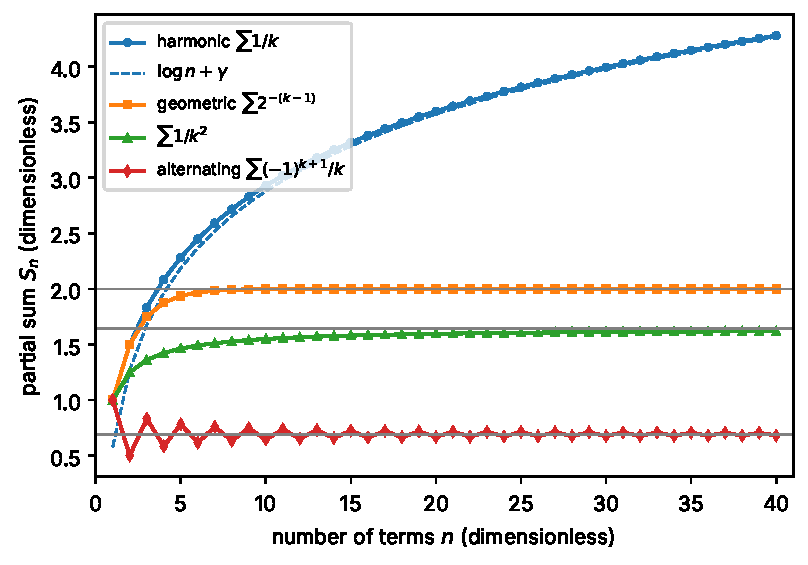
\includegraphics[width=0.85\linewidth]{figs/series_partialsums.pdf}
\caption{Partial sums $S_n$ of four series for $n=1$ to $40$. The geometric series $\sum_{k\ge1}2^{-(k-1)}$ approaches $2$ very quickly; $\sum 1/k^2$ approaches $\pi^2/6=1.644934$ slowly (tail about $1/n$); the alternating harmonic series zigzags around $\log2=0.693147$; the harmonic series $\sum1/k$ grows without bound, following $\log n+\gamma$ with $\gamma=0.577216$. Horizontal gray lines mark the limits.}
\label{fig:series-partialsums}
\end{figure}

\begin{pycode}
import numpy as np
# partial sums of the geometric series with ratio r
r = 2**-0.5
k = np.arange(0, 30)
S = np.cumsum(r**k)          # S[n-1] = sum of first n terms
print(S[16], 1/(1 - r))       # 17 terms vs exact sum 2+sqrt(2)
print(1/(1 - r) - S[16])      # tail after 17 terms, below 0.01
\end{pycode}

\begin{checkpoint}
For which complex numbers $r$ does $\sum_{k=0}^\infty r^k$ converge? Does it converge for $r=e^{i\theta}/2$?
\end{checkpoint}
\checkanswer{Exactly for $\abs r<1$. For $r=e^{i\theta}/2$, $\abs r=\tfrac12$, so it converges, to $1/(1-e^{i\theta}/2)$, for every real $\theta$.}

\begin{keyideas}
\item A series converges when its sequence of partial sums $S_n$ converges; the tail $S-S_n$ is the truncation error.
\item If a series converges, its terms tend to zero; the converse is false.
\item $\sum_{k=0}^{n-1}r^k=(1-r^n)/(1-r)$ exactly (Eq.~\eqref{eq:series-geom-partial}); for $\abs r<1$ the sum is $1/(1-r)$ and the tail is $r^n/(1-r)$ (Eqs.~\eqref{eq:series-geom-sum}, \eqref{eq:series-geom-tail}). This holds for complex $r$.
\end{keyideas}

\section{Telescoping sums}\label{sec:series-telescoping}

Some sums collapse like a pocket telescope. Suppose each term is a difference of consecutive members of another sequence, $a_k=b_k-b_{k+1}$. Then
\begin{align}
\sum_{k=1}^{n}(b_k-b_{k+1})
&=(b_1-b_2)+(b_2-b_3)+\cdots+(b_n-b_{n+1})\nonumber\\
&=b_1-b_{n+1},
\label{eq:series-telescope}
\end{align}
because each of $b_2,\dots,b_n$ appears once with a plus sign and once with a minus sign. Therefore the series $\sum_{k=1}^\infty(b_k-b_{k+1})$ converges if and only if $b_n$ converges, and then its sum is $b_1-\lim_{n\to\infty}b_n$.

\emph{Example 1.} Since
\[
\frac1k-\frac1{k+1}=\frac{(k+1)-k}{k(k+1)}=\frac{1}{k(k+1)},
\]
Eq.~\eqref{eq:series-telescope} with $b_k=1/k$ gives $\sum_{k=1}^n\frac{1}{k(k+1)}=1-\frac1{n+1}\to1$. So $\sum_{k=1}^\infty\frac{1}{k(k+1)}=1$.

\emph{Example 2.} With $b_k=-\log k$ we have $b_k-b_{k+1}=\log(k+1)-\log k=\log\frac{k+1}{k}=\log\left(1+\frac1k\right)$. Hence
\[
\sum_{k=1}^n\log\left(1+\frac1k\right)=-\log1+\log(n+1)=\log(n+1)\to\infty .
\]
The terms $\log(1+1/k)$ tend to $0$, yet the series diverges: a second warning that the term test is not a convergence test.

\begin{sample}{A telescoping sum with a gap}
Find $\sum_{k=2}^{\infty}\dfrac{1}{k^2-1}$.

\textbf{Step 1 (partial fractions):} $k^2-1=(k-1)(k+1)$, and
\[
\frac{1}{k-1}-\frac1{k+1}=\frac{(k+1)-(k-1)}{(k-1)(k+1)}=\frac{2}{k^2-1},
\]
so $\dfrac1{k^2-1}=\dfrac12\left(\dfrac1{k-1}-\dfrac1{k+1}\right)$.

\textbf{Step 2 (write out the partial sum):}
\[
\sum_{k=2}^{n}\left(\frac1{k-1}-\frac1{k+1}\right)
=\left[\frac11+\frac12+\cdots+\frac1{n-1}\right]-\left[\frac13+\frac14+\cdots+\frac1{n+1}\right].
\]

\textbf{Step 3 (cancel):} The terms $1/3,\dots,1/(n-1)$ appear in both brackets. What survives is $1+\tfrac12-\tfrac1n-\tfrac1{n+1}$.

\textbf{Step 4 (limit):} So $\sum_{k=2}^n\frac1{k^2-1}=\frac12\left(\frac32-\frac1n-\frac1{n+1}\right)\to\frac34$. For instance at $n=10$ the partial sum is $\tfrac12(1.5-0.1-0.090909)=0.654545$, still far from the limit.

\[\boxed{\sum_{k=2}^\infty\frac{1}{k^2-1}=\frac34}\]
\end{sample}

\begin{checkpoint}
The terms of $\sum_{k=1}^\infty\log(1+1/k)$ tend to zero. Does the series converge?
\end{checkpoint}
\checkanswer{No. It telescopes to $\log(n+1)$, which grows without bound.}

\begin{keyideas}
\item $\sum_{k=1}^n(b_k-b_{k+1})=b_1-b_{n+1}$ (Eq.~\eqref{eq:series-telescope}); the series converges exactly when $b_n$ does.
\item Partial fractions turn many rational sums into telescoping ones.
\end{keyideas}

\section{The harmonic series diverges}\label{sec:series-harmonic}

The \textbf{harmonic series} is $\sum_{k=1}^\infty\frac1k$, and its partial sums are the \textbf{harmonic numbers} $H_n=\sum_{k=1}^n\frac1k$. The name comes from music: a string fixed at both ends and vibrating in its $k$-th harmonic has a wavelength equal to $1/k$ of the fundamental wavelength (standing waves, HRW~\cite{hrw}), so the relative wavelengths $1,\tfrac12,\tfrac13,\dots$ are the terms of the series.

\subsection{Oresme's proof}

\textbf{Theorem.} The harmonic series diverges: $H_n\to\infty$.

\emph{Proof.} Group the terms of $H_{2^K}$ into blocks:
\[
H_{2^K}=1+\underbrace{\tfrac12}_{\text{block }1}+\underbrace{\left(\tfrac13+\tfrac14\right)}_{\text{block }2}+\underbrace{\left(\tfrac15+\cdots+\tfrac18\right)}_{\text{block }3}+\cdots+\underbrace{\left(\tfrac1{2^{K-1}+1}+\cdots+\tfrac1{2^K}\right)}_{\text{block }K}.
\]
Block $j$ runs from $1/(2^{j-1}+1)$ to $1/2^j$, so it contains $2^j-2^{j-1}=2^{j-1}$ terms, and each of them is at least the smallest one, $1/2^j$. Hence block $j$ is at least $2^{j-1}\times 1/2^j=\tfrac12$. Adding the $K$ blocks and the leading 1,
\begin{equation}
H_{2^K}\ge1+\frac K2 .
\label{eq:series-oresme}
\end{equation}
Given any bound $B$, choose an integer $K>2(B-1)$. Then $H_{2^K}>B$, and since $H_n$ increases with $n$ (all terms are positive), $H_n>B$ for all $n\ge2^K$. So $H_n\to\infty$. $\square$

For example $H_8=1+\tfrac12+\cdots+\tfrac18=2.717857$, while Eq.~\eqref{eq:series-oresme} with $K=3$ guarantees only $H_8\ge2.5$.

\subsection{How fast does $H_n$ grow?}

Compare the sum with an integral. On the interval $k\le x\le k+1$ we have $1/x\le1/k$, so
\[
\int_k^{k+1}\frac{\dd x}{x}\le\frac1k .
\]
Summing over $k=1,\dots,n$, the integrals join into one: $\int_1^{n+1}\dd x/x=\log(n+1)\le H_n$. Similarly, on $k-1\le x\le k$ we have $1/x\ge1/k$, so $1/k\le\int_{k-1}^k\dd x/x$; summing over $k=2,\dots,n$ gives $H_n-1\le\int_1^n\dd x/x=\log n$. Together,
\begin{equation}
\log(n+1)\le H_n\le1+\log n .
\label{eq:series-harmonic-bounds}
\end{equation}
So $H_n$ grows like $\log n$: without bound, but extremely slowly. At $n=10$: $\log 11=2.397895\le H_{10}=2.928968\le1+\log10=3.302585$.

\subsection{The Euler--Mascheroni constant}

Let $g_n=H_n-\log n$. Two facts:

\emph{(i) $g_n$ decreases.} Compute
\[
g_{n+1}-g_n=\frac1{n+1}-\bigl[\log(n+1)-\log n\bigr]=\frac1{n+1}-\int_n^{n+1}\frac{\dd x}{x}.
\]
On $n\le x<n+1$ we have $1/x>1/(n+1)$, so the integral exceeds $\int_n^{n+1}\frac{\dd x}{n+1}=\frac1{n+1}$. Hence $g_{n+1}-g_n<0$.

\emph{(ii) $g_n$ is bounded below by $0$.} By Eq.~\eqref{eq:series-harmonic-bounds}, $g_n\ge\log(n+1)-\log n>0$.

A decreasing sequence bounded below converges (monotone convergence, \cref{sec:series-sequences}). Its limit is the \textbf{Euler--Mascheroni constant}
\begin{equation}
\gamma=\lim_{n\to\infty}\bigl(H_n-\log n\bigr)=0.5772156649\ldots
\label{eq:series-gamma}
\end{equation}
(The digits are a standard constant; our proof shows only that $0\le\gamma\le g_1=1$.) At $n=10$, $g_{10}=2.928968-2.302585=0.626383$, still decreasing toward $\gamma$.

\begin{beyond}
\textbf{A sharper form of $H_n$ (proved; proof beyond this book).} The Euler--Maclaurin summation formula, a refined comparison of sums with integrals, gives
\[
H_n=\log n+\gamma+\frac1{2n}+\order(n^{-2}),
\]
where $\order(n^{-2})$ denotes a remainder whose size is at most a constant times $n^{-2}$ for all large $n$ (big-O notation, treated in Chapter~\ref{ch:asymptotics}). We do not prove it here; see Riley, Hobson and Bence~\cite{rhb} or Apostol~\cite{apostol}. We use it only to estimate numbers, never inside a proof.
\end{beyond}

\begin{sample}{When does $H_n$ first exceed 10?}
Estimate the smallest $n$ with $H_n>10$, first from Oresme's bound and then from $\gamma$.

\textbf{Step 1 (Oresme):} Eq.~\eqref{eq:series-oresme} gives $H_{2^K}\ge1+K/2$. Setting $1+K/2=10$ gives $K=18$. The inequality is in fact strict for $K\ge2$, because block 2 is $\tfrac13+\tfrac14>\tfrac12$. So $H_{2^{18}}>10$, and $n=2^{18}=262144$ certainly works. This is a guarantee, not an estimate.

\textbf{Step 2 (with $\gamma$):} Using $H_n\approx\log n+\gamma$, solve $\log n+\gamma=10$: $n\approx e^{10-\gamma}=e^{9.4227843}\approx12367$.

\textbf{Step 3 (exact check):} Summing directly on a computer (a short numpy loop of the kind used in Problem~19) gives $H_{12366}<10<H_{12367}$.

\[\boxed{n=12367}\]
Oresme's bound is about 21 times too pessimistic, but it is a proof; the $\gamma$ estimate is accurate because, by the sharper form quoted in the box above, the error of $H_n\approx\log n+\gamma$ is about $1/(2n)$, only $4\times10^{-5}$ here.
\end{sample}

The same estimate shows how slowly the harmonic series diverges. To pass $100$ you need about $e^{100-\gamma}\approx1.5\times10^{43}$ terms, far more than any computer could add. Oresme's grouping argument, made in the fourteenth century, proves divergence. Direct summation, by contrast, never gets far enough to show it. A truncated sum can look convergent long before it reveals its true nature.

\begin{keyideas}
\item The harmonic series diverges (Oresme, Eq.~\eqref{eq:series-oresme}), although its terms tend to zero.
\item $\log(n+1)\le H_n\le1+\log n$ (Eq.~\eqref{eq:series-harmonic-bounds}); $H_n-\log n\to\gamma=0.5772\ldots$ (Eq.~\eqref{eq:series-gamma}).
\item Comparing a sum with an integral, rectangle by rectangle, gives two-sided bounds. This idea is the integral test of the next section.
\end{keyideas}

\section{Series of positive terms: comparison and the integral test}\label{sec:series-positive}

When all terms are nonnegative, the partial sums can only increase. Monotone convergence then says: \emph{a series of nonnegative terms converges if and only if its partial sums are bounded.} (If they are bounded, they converge; if not, they exceed every bound and the series diverges to $+\infty$.) This single fact powers the two tests below.

\subsection{The comparison test}

\textbf{Theorem (comparison).} Suppose $0\le a_k\le b_k$ for all $k$. If $\sum b_k$ converges, then $\sum a_k$ converges and $\sum a_k\le\sum b_k$. If $\sum a_k$ diverges, then $\sum b_k$ diverges.

\emph{Proof.} Let $B=\sum_{k=1}^\infty b_k$. Since the $b_k$ are nonnegative, every partial sum of the $b$'s is at most $B$. Then $\sum_{k=1}^n a_k\le\sum_{k=1}^n b_k\le B$, so the partial sums of $\sum a_k$ are bounded, hence converge, and the limit is at most $B$. The second statement is the first one read backwards: if $\sum b_k$ converged, $\sum a_k$ would too. $\square$

Finitely many terms never affect convergence (they change every partial sum beyond some point by the same fixed amount), so it is enough that $0\le a_k\le b_k$ for all $k$ beyond some $K$.

\emph{Example.} For $k\ge2$, $k^2\ge k(k-1)$, so $1/k^2\le1/(k(k-1))$. The comparison series $\sum_{k=2}^\infty\frac1{k(k-1)}=\sum_{j=1}^\infty\frac1{j(j+1)}=1$ (substitute $j=k-1$ and use \cref{sec:series-telescoping}). Therefore $\sum_{k=1}^\infty\frac1{k^2}\le1+1=2$: the series converges.

\emph{Example.} $1/\sqrt k\ge1/k$ for $k\ge1$, and $\sum1/k$ diverges, so $\sum1/\sqrt k$ diverges.

\subsection{The integral test}

We write $\int_a^\infty f(x)\,\dd x$ for $\lim_{K\to\infty}\int_a^K f(x)\,\dd x$ when that limit exists (an \textbf{improper integral}).

\textbf{Theorem (integral test).} Let $f$ be continuous, positive and decreasing on $[1,\infty)$, and let $a_k=f(k)$. Then for every $n\ge1$
\begin{equation}
\int_1^{n+1}f(x)\,\dd x\;\le\;\sum_{k=1}^{n}f(k)\;\le\;f(1)+\int_1^{n}f(x)\,\dd x,
\label{eq:series-integral-test}
\end{equation}
and the series $\sum_{k=1}^\infty f(k)$ converges if and only if the integrals $\int_1^nf(x)\,\dd x$ stay bounded as $n\to\infty$. Moreover, when the series converges, its tail after $n$ terms satisfies
\begin{equation}
\int_{n+1}^{\infty}f(x)\,\dd x\;\le\;\sum_{k=n+1}^{\infty}f(k)\;\le\;\int_{n}^{\infty}f(x)\,\dd x .
\label{eq:series-tail-bounds}
\end{equation}

\emph{Proof.} Because $f$ decreases, on the interval $[k,k+1]$ we have $f(x)\le f(k)$, so $\int_k^{k+1}f\,\dd x\le f(k)$: the rectangle of height $f(k)$ and width 1 lies above the curve (\cref{fig:series-integraltest}, left). Summing $k=1,\dots,n$ gives the left inequality of Eq.~\eqref{eq:series-integral-test}. On $[k-1,k]$ we have $f(x)\ge f(k)$, so $f(k)\le\int_{k-1}^kf\,\dd x$: the rectangle lies below the curve (\cref{fig:series-integraltest}, right). Summing $k=2,\dots,n$ gives $\sum_{k=2}^nf(k)\le\int_1^nf\,\dd x$; adding $f(1)$ gives the right inequality.

If $\int_1^nf\le I$ for all $n$, the right inequality bounds the partial sums by $f(1)+I$, so the series converges. If the integrals are unbounded (they increase with $n$ because $f>0$), the left inequality shows the partial sums are unbounded, so the series diverges.

For the tail, sum the same rectangle inequalities over $k=n+1,\dots,K$ and let $K\to\infty$: $\int_k^{k+1}f\le f(k)$ summed gives $\int_{n+1}^{K+1}f\le\sum_{n+1}^{K}f(k)$, and $f(k)\le\int_{k-1}^kf$ summed gives $\sum_{n+1}^{K}f(k)\le\int_n^{K}f$. Taking $K\to\infty$ in both gives Eq.~\eqref{eq:series-tail-bounds}. The improper integrals in it exist. For positive $f$ the integrals $\int_a^Kf\,\dd x$ increase with $K$. When the series converges with sum $S$, they are bounded, because the left inequality of Eq.~\eqref{eq:series-integral-test} gives $\int_1^{K+1}f\,\dd x\le S$. Monotone convergence then applies. $\square$

\begin{figure}[htbp]\centering
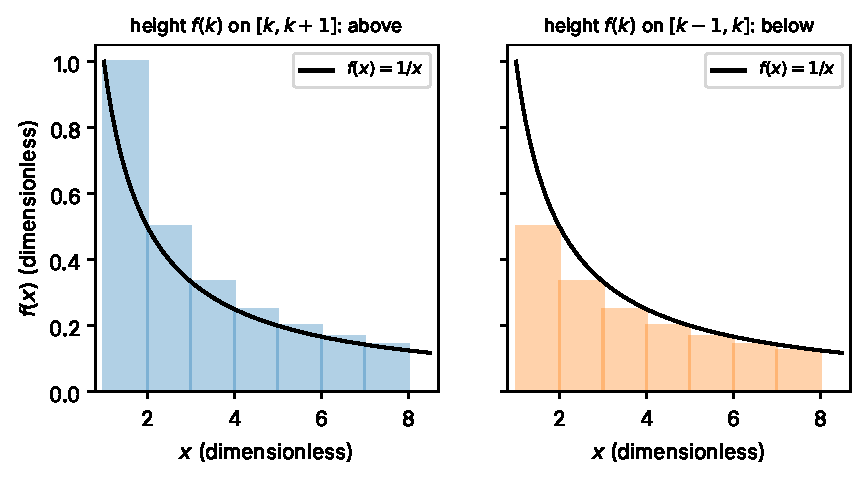
\includegraphics[width=0.85\linewidth]{figs/series_integraltest.pdf}
\caption{The integral test for $f(x)=1/x$. Left: rectangles of height $f(k)$ on $[k,k+1]$ lie above the curve, so $\sum_{k=1}^{7}f(k)\ge\int_1^8f\,\dd x$. Right: rectangles of height $f(k)$ on $[k-1,k]$ lie below the curve, so $\sum_{k=2}^{8}f(k)\le\int_1^8f\,\dd x$. Squeezing the sum between two integrals gives Eqs.~\eqref{eq:series-integral-test} and~\eqref{eq:series-tail-bounds}.}
\label{fig:series-integraltest}
\end{figure}

\subsection{The $p$-series $\sum k^{-s}$ for real $s$}

Series of the form $\sum k^{-s}$ are traditionally called \textbf{$p$-series}, because the exponent is often written $p$. We write $s$ instead and keep $p$ for primes.

\textbf{Theorem.} For real $s$, the series $\sum_{k=1}^\infty k^{-s}$ converges if and only if $s>1$.

\emph{Proof.} If $s\le0$, then $k^{-s}=k^{\abs s}\ge1$ for all $k$, the terms do not tend to zero, and the series diverges. If $s>0$, $f(x)=x^{-s}$ is positive, continuous and decreasing on $[1,\infty)$ (its derivative $-sx^{-s-1}$ is negative), so the integral test applies. For $s\ne1$,
\[
\int_1^nx^{-s}\,\dd x=\left[\frac{x^{1-s}}{1-s}\right]_1^n=\frac{n^{1-s}-1}{1-s},
\]
and for $s=1$ the integral is $\log n$.
\begin{itemize}
\item If $s>1$, then $1-s<0$, $n^{1-s}\to0$, and the integral tends to $\frac{-1}{1-s}=\frac{1}{s-1}$: bounded. The series converges.
\item If $0<s<1$, then $1-s>0$, $n^{1-s}\to\infty$: unbounded. The series diverges.
\item If $s=1$, $\log n\to\infty$: the harmonic series diverges (as already shown).
\end{itemize}
$\square$

For $s>1$ the sum is denoted
\begin{equation}
\zeta(s)=\sum_{k=1}^\infty\frac1{k^{s}}\qquad(s>1),
\label{eq:series-pseries}
\end{equation}
the Riemann zeta function on the real axis; Chapter~\ref{ch:zeta} studies it in depth. Eq.~\eqref{eq:series-tail-bounds} gives the tail after $n$ terms:
\[
\frac{(n+1)^{1-s}}{s-1}\le\zeta(s)-\sum_{k=1}^nk^{-s}\le\frac{n^{1-s}}{s-1}.
\]

\begin{sample}{Bracketing $\zeta(2)$}
Compute $S_{10}=\sum_{k=1}^{10}1/k^2$ and use Eq.~\eqref{eq:series-tail-bounds} to bracket $\zeta(2)$. Compare with the known value $\zeta(2)=\pi^2/6$ (Euler's result; it follows from Parseval's theorem applied to a suitable Fourier series, the tool of Chapter~\ref{ch:fourier-series}, and here we take it as a known value).

\textbf{Step 1:} $S_{10}=1+0.25+0.111111+0.0625+0.04+0.027778+0.020408+0.015625+0.012346+0.01=1.549768$.

\textbf{Step 2:} With $f(x)=x^{-2}$, $\int_a^\infty x^{-2}\,\dd x=1/a$. So the tail lies between $1/11=0.090909$ and $1/10=0.1$.

\textbf{Step 3:} Therefore $1.549768+0.090909\le\zeta(2)\le1.549768+0.1$.

\[\boxed{1.640677\le\zeta(2)\le1.649768}\]
The true value $\pi^2/6=1.644934$ lies inside. The midpoint of the bracket, $1.645222$, is off by only $0.00029$, much better than $S_{10}$ itself (off by $0.095$). Averaging works so well because the two integral bounds err in opposite directions: the lower bound misses the true tail by the small curved slivers between the rectangles and the curve on one side, the upper bound overshoots by similar slivers on the other side, and for a slowly varying $f$ these nearly cancel in the average.
\end{sample}

\begin{sample}{How fast does $\sum k^{-1/2}$ diverge?}
On the critical line $\Re s=\tfrac12$ (Chapter~\ref{ch:zeta}) the terms of $\sum k^{-s}$ have modulus $k^{-1/2}$. Bound $\sum_{k=1}^{1000}k^{-1/2}$.

\textbf{Step 1:} $f(x)=x^{-1/2}$ is positive and decreasing, with $\int_a^bx^{-1/2}\,\dd x=2(\sqrt b-\sqrt a)$.

\textbf{Step 2:} Eq.~\eqref{eq:series-integral-test} with $n=1000$: lower bound $2(\sqrt{1001}-1)=2(31.638584-1)=61.277168$; upper bound $1+2(\sqrt{1000}-1)=1+2(30.622777)=62.245553$.

\[\boxed{61.277\le\sum_{k=1}^{1000}k^{-1/2}\le62.246}\]
(Direct summation gives $61.801$.) The sum grows like $2\sqrt n$: by $n=10^6$ it is near 2000. A sum of moduli this large tells you that cancellation between terms, not the size of the terms, would have to do all the work on the critical line.
\end{sample}

\begin{checkpoint}
Does $\sum_{k=1}^\infty k^{-1.5}$ converge? Bound the tail after 100 terms.
\end{checkpoint}
\checkanswer{Yes, since $1.5>1$. By Eq.~\eqref{eq:series-tail-bounds} the tail is at most $\int_{100}^\infty x^{-1.5}\,\dd x=2/\sqrt{100}=0.2$. Convergence is slow: the tail decays only like $2/\sqrt n$.}

\begin{keyideas}
\item A series of nonnegative terms converges if and only if its partial sums are bounded.
\item Comparison: smaller than a convergent series converges; larger than a divergent series diverges.
\item Integral test: for positive decreasing $f$, $\sum f(k)$ and $\int f$ converge or diverge together, and integrals bracket the tail (Eqs.~\eqref{eq:series-integral-test}, \eqref{eq:series-tail-bounds}).
\item $\sum k^{-s}$ converges exactly for $s>1$; the tail after $n$ terms is about $n^{1-s}/(s-1)$.
\end{keyideas}

\section{Absolute convergence and complex series}\label{sec:series-absolute}

\subsection{Definition and the main theorem}

A series $\sum a_k$ (real or complex terms) \textbf{converges absolutely} if the series of moduli $\sum\abs{a_k}$ converges. A series that converges but not absolutely is said to \textbf{converge conditionally}.

We need the triangle inequality for complex numbers, $\abs{z+w}\le\abs z+\abs w$. Here is a short proof. Using $\abs u^2=u\bar u$,
\begin{align*}
\abs{z+w}^2&=(z+w)(\bar z+\bar w)=\abs z^2+\abs w^2+z\bar w+\bar zw\\
&=\abs z^2+\abs w^2+2\Re(z\bar w)\qquad(\text{since } \bar zw=\overline{z\bar w})\\
&\le\abs z^2+\abs w^2+2\abs{z\bar w}\qquad(\Re u\le\abs u)\\
&=(\abs z+\abs w)^2\qquad(\abs{z\bar w}=\abs z\abs w).
\end{align*}
Taking square roots gives the inequality. By induction it extends to $\abs{\sum_{k=1}^na_k}\le\sum_{k=1}^n\abs{a_k}$.

\textbf{Theorem.} An absolutely convergent series converges, and
\begin{equation}
\Bigl|\sum_{k=1}^\infty a_k\Bigr|\le\sum_{k=1}^\infty\abs{a_k}.
\label{eq:series-abs-ineq}
\end{equation}

\emph{Proof for real terms.} Let $b_k=a_k+\abs{a_k}$. Then $0\le b_k\le2\abs{a_k}$ (if $a_k\ge0$, $b_k=2a_k$; if $a_k<0$, $b_k=0$). Since $\sum2\abs{a_k}$ converges, so does $\sum b_k$ by comparison. Now $a_k=b_k-\abs{a_k}$, so the partial sums of $\sum a_k$ are differences of the partial sums of two convergent series, and therefore converge.

\emph{Proof for complex terms.} Write $a_k=x_k+iy_k$. Since $\abs{x_k}\le\abs{a_k}$ and $\abs{y_k}\le\abs{a_k}$, comparison shows that $\sum x_k$ and $\sum y_k$ converge absolutely, hence converge by the real case. The complex partial sums then converge because their real and imaginary parts do (\cref{sec:series-sequences}).

\emph{The inequality.} For each $n$, the finite triangle inequality gives $\abs{S_n}\le\sum_{k=1}^n\abs{a_k}\le\sum_{k=1}^\infty\abs{a_k}$. Let $n\to\infty$; $\abs{S_n}\to\abs S$ by continuity of the modulus. $\square$

The practical value of Eq.~\eqref{eq:series-abs-ineq}: applied to the tail, it says
\[
\Bigl|\sum_{k=n+1}^\infty a_k\Bigr|\le\sum_{k=n+1}^\infty\abs{a_k},
\]
so the truncation error of an absolutely convergent series is controlled by the moduli alone, whatever the phases do.

\subsection{Rearranging an absolutely convergent series}

A \textbf{rearrangement} of $\sum a_k$ is a series $\sum_j a_{q(j)}$ in which the reordering $q$ lists every positive integer exactly once in some new order (so $q(1),q(2),\dots$ is a shuffled copy of $1,2,\dots$). For finite sums the order never matters. For infinite sums it can matter (\cref{sec:series-alternating}), but not when the series converges absolutely.

\textbf{Theorem.} If $\sum a_k$ converges absolutely to $S$, every rearrangement converges absolutely to the same $S$.

\emph{Proof.} First suppose all $a_k\ge0$. Take any partial sum $T_J=\sum_{j=1}^Ja_{q(j)}$ of the rearranged series. It uses finitely many terms of the original series, all with index at most $K=\max(q(1),\dots,q(J))$, so $T_J\le S_K\le S$ (adding the missing nonnegative terms only increases the sum). So the rearranged partial sums are bounded by $S$, increase, and converge to some $T\le S$. The original series is in turn a rearrangement of the new one, so the same argument gives $S\le T$. Hence $T=S$.

For real terms of either sign, write $a_k=b_k-\abs{a_k}$ with $b_k=a_k+\abs{a_k}\ge0$ as before; both $\sum b_k$ and $\sum\abs{a_k}$ are nonnegative convergent series, each rearrangement of them has the same sum, so the rearrangement of $\sum a_k$ has sum $\sum b_k-\sum\abs{a_k}=S$. For complex terms apply this to real and imaginary parts. $\square$

\subsection{The Dirichlet series $\sum k^{-s}$ for complex $s$}

A series of the form $\sum_kc_kk^{-s}$ is called a \textbf{Dirichlet series}; here all $c_k=1$.


Recall from Chapter~\ref{ch:complex} that for a positive integer $k$ and a complex number $s=\sigma+it$ ($\sigma,t$ real),
\[
k^{-s}=e^{-s\log k}=e^{-\sigma\log k}\,e^{-it\log k}=k^{-\sigma}e^{-it\log k},
\]
so that
\begin{equation}
\abs{k^{-s}}=k^{-\sigma}.
\label{eq:series-ks-modulus}
\end{equation}
The modulus depends only on the real part $\sigma$; the imaginary part $t$ only rotates the phase, at angular frequency $\log k$ in $t$.

\textbf{Theorem.} For $\Re s=\sigma>1$, the series $\sum_{k=1}^\infty k^{-s}$ converges absolutely, and its sum $\zeta(s)$ satisfies, for every $n\ge1$,
\begin{equation}
\Bigl|\zeta(s)-\sum_{k=1}^nk^{-s}\Bigr|\le\frac{n^{1-\sigma}}{\sigma-1}.
\label{eq:series-zeta-tail}
\end{equation}

\emph{Proof.} By Eq.~\eqref{eq:series-ks-modulus}, $\sum\abs{k^{-s}}=\sum k^{-\sigma}$, which converges for $\sigma>1$ (\cref{sec:series-positive}). The tail bound is Eq.~\eqref{eq:series-abs-ineq} applied to the tail, followed by Eq.~\eqref{eq:series-tail-bounds} with $f(x)=x^{-\sigma}$. $\square$

\begin{sample}{Truncating $\zeta(s)$ off the real axis}
Take $s=2+i\,t_1$ with $t_1=14.134725$ (RE1). How many terms guarantee that the partial sum is within $0.01$ of $\zeta(s)$?

\textbf{Step 1:} Here $\sigma=2$. Eq.~\eqref{eq:series-zeta-tail} gives $\abs{\zeta(s)-S_n}\le n^{1-2}/(2-1)=1/n$.

\textbf{Step 2:} $1/n\le0.01$ requires $n\ge100$.

\[\boxed{n=100\ \text{terms suffice}}\]
Notice that the bound does not depend on $t$ at all. Whether $t$ is $14$ or $10^6$, absolute convergence controls the error through the moduli $k^{-2}$ alone. (Computing the 100-term sum and comparing it with \texttt{mpmath.zeta} confirms that the actual error at $n=100$ is below $0.01$.)
\end{sample}

\subsection{What happens on the critical line}

At $\sigma=\tfrac12$ the moduli are $k^{-1/2}$, whose sum diverges (the $p$-series theorem with $s=\tfrac12$; see also the Sample Problem ``How fast does $\sum k^{-1/2}$ diverge?'' in \cref{sec:series-positive}). So the series is not absolutely convergent there. Does it at least converge conditionally? The terms do tend to zero, so the term test is silent. The answer is no.

\begin{beyond}
\textbf{Partial sums of $\sum k^{-s}$ for $0<\sigma<1$ (proved; proof beyond this book).} Fix $s=\sigma+it$ with $0<\sigma<1$. Then, as $n\to\infty$,
\[
\sum_{k=1}^nk^{-s}=\zeta(s)+\frac{n^{1-s}}{1-s}+\frac12n^{-s}+\epsilon_n,\qquad\epsilon_n\to0,
\]
where $\zeta(s)$ is the analytically continued zeta function of Chapter~\ref{ch:zeta}, and $\abs{\epsilon_n}$ is small compared with $\tfrac12 n^{-\sigma}$ once $n$ is large compared with $\abs t$. The proof uses Euler--Maclaurin summation; see Titchmarsh~\cite{titchmarsh}, in the discussion of approximate formulas for $\zeta(s)$ in the critical strip, or Edwards~\cite{edwards}. Since $\abs{n^{1-s}}=n^{1-\sigma}\to\infty$, the partial sums do not converge: the series diverges everywhere in $0<\sigma<1$, including the critical line.
\end{beyond}

\Cref{fig:series-spiral} shows both regimes. At $s=2+it_1$ the partial sums wind briefly and settle on a point. At the first zero $s=\rho_1=\tfrac12+it_1$, where $\zeta(\rho_1)=0$, the beyond box predicts $S_n\approx n^{1-s}/(1-s)$: a spiral around the origin with radius $\sqrt n/\abs{1-s}$ growing without bound. More precisely, because $\zeta(\rho_1)=0$, the box gives $S_n-\frac{n^{1-s}}{1-s}=\tfrac12n^{-s}+\epsilon_n$, whose modulus should be close to $\abs{\tfrac12n^{-s}}=\tfrac12n^{-1/2}$. Numerically, at $n=1000$ the radius is $\sqrt{1000}/14.1436=2.236$, and $\abs{S_{1000}-1000^{1-s}/(1-s)}$ is about $0.016$, matching $\tfrac12\cdot1000^{-1/2}=0.0158$ (a numerical observation; the listing below computes it).

\begin{figure}[htbp]\centering
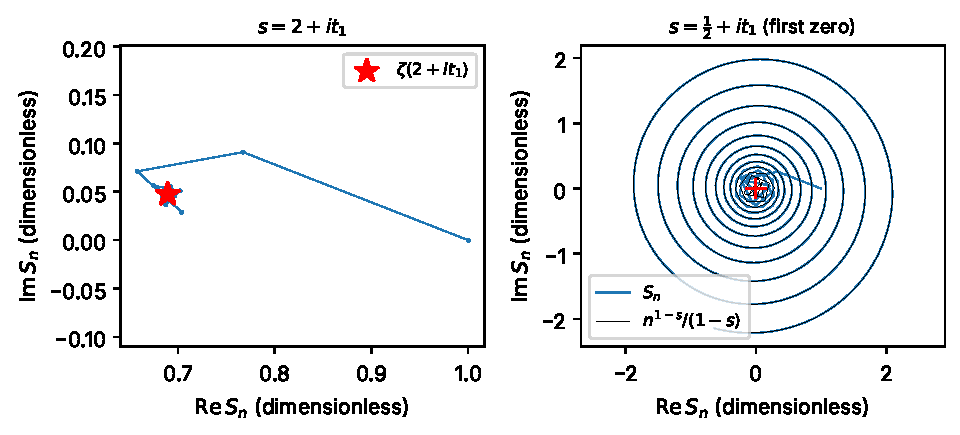
\includegraphics[width=0.85\linewidth]{figs/series_spiral.pdf}
\caption{Partial sums $S_n=\sum_{k=1}^nk^{-s}$ in the complex plane. Left: $s=2+i\,t_1$ with $t_1=14.134725$; the series converges absolutely and the partial sums settle on $\zeta(s)$ (star). Right: $s=\tfrac12+i\,t_1$, the first nontrivial zero; the partial sums spiral outward around the origin, following the curve $n^{1-s}/(1-s)$ (thin line), and never converge, although $\zeta(\tfrac12+it_1)=0$.}
\label{fig:series-spiral}
\end{figure}

\begin{pycode}
import numpy as np, qmnt
t1 = qmnt.zeros(1)[0]
s = 0.5 + 1j*t1                       # first zero rho_1
k = np.arange(1, 1001)
S = np.cumsum(np.exp(-s*np.log(k)))   # partial sums of k^(-s)
main = k**(1 - s) / (1 - s)           # growing spiral term
print(abs(S[-1]), np.sqrt(1000)/abs(1 - s))
print(abs(S[-1] - main[-1]))          # about 0.016
\end{pycode}

\begin{checkpoint}
Is $\sum_{k=1}^\infty k^{-s}$ absolutely convergent at $s=1.5+100i$? At $s=0.5+100i$?
\end{checkpoint}
\checkanswer{At $s=1.5+100i$ yes: the moduli are $k^{-1.5}$, and $1.5>1$; the value of $t$ is irrelevant. At $s=0.5+100i$ no: the moduli $k^{-0.5}$ sum to infinity, and by the beyond box the series does not converge at all.}

\begin{keyideas}
\item Absolute convergence ($\sum\abs{a_k}<\infty$) implies convergence, with $\abs{\sum a_k}\le\sum\abs{a_k}$ (Eq.~\eqref{eq:series-abs-ineq}); the tail is bounded by the moduli alone.
\item Absolutely convergent series may be rearranged freely without changing the sum.
\item $\abs{k^{-s}}=k^{-\sigma}$, so $\sum k^{-s}$ converges absolutely for $\Re s>1$, with tail at most $n^{1-\sigma}/(\sigma-1)$ (Eq.~\eqref{eq:series-zeta-tail}), independent of $t$.
\item On the critical line the Dirichlet series diverges; its partial sums spiral outward. The zeros of $\zeta$ cannot be found by summing $\sum k^{-s}$ there.
\end{keyideas}

\section{Conditional convergence and alternating series}\label{sec:series-alternating}
% DYK-BEGIN
\begin{didyouknow}{Rearrange to Any Answer}
Bernhard Riemann proved that a conditionally convergent series can be rearranged to add up to \emph{any} real number you choose, or even to diverge. The alternating harmonic series $1-\tfrac12+\tfrac13-\cdots$ sums to $\log 2$. Reorder the terms as two positives, then one negative, and the sum becomes $\tfrac32\log 2$. The result is in his 1854 habilitation thesis on trigonometric series, published only after his death.
\end{didyouknow}
% DYK-END

\subsection{The alternating series test}

When terms alternate in sign, cancellation can make a series converge even though the moduli sum to infinity.

\textbf{Theorem (alternating series test).} Let $a_1\ge a_2\ge a_3\ge\cdots\ge0$ with $a_k\to0$. Then $\sum_{k=1}^\infty(-1)^{k+1}a_k=a_1-a_2+a_3-\cdots$ converges to a sum $S$, and for every $n$
\begin{equation}
\abs{S-S_n}\le a_{n+1}.
\label{eq:series-alt-error}
\end{equation}

\emph{Proof.} Look at even and odd partial sums separately.
\begin{itemize}
\item $S_{2n+2}-S_{2n}=a_{2n+1}-a_{2n+2}\ge0$: the even partial sums increase.
\item $S_{2n+1}-S_{2n-1}=-a_{2n}+a_{2n+1}\le0$: the odd partial sums decrease.
\item $S_{2n}=S_{2n-1}-a_{2n}\le S_{2n-1}$: each even sum lies below the preceding odd sum.
\end{itemize}
Combining these, $S_2\le S_4\le\cdots\le S_{2n}\le S_{2n-1}\le\cdots\le S_3\le S_1$. The even sums increase and are bounded above by $S_1$, so they converge to some $E$; the odd sums decrease and are bounded below by $S_2$, so they converge to some $O$ (monotone convergence). Their difference is $O-E=\lim(S_{2n-1}-S_{2n})=\lim a_{2n}=0$, so $O=E=S$. Given $\varepsilon$, choose $N$ so that both the even and the odd sums beyond $N$ lie within $\varepsilon$ of $S$; then all partial sums beyond $N$ do, so $S_n\to S$.

Finally, $S$ is at least every even partial sum and at most every odd one. Consecutive partial sums $S_n$, $S_{n+1}$ are one even and one odd, so $S$ lies between them, and $\abs{S-S_n}\le\abs{S_{n+1}-S_n}=a_{n+1}$. $\square$

The \textbf{alternating harmonic series} $1-\tfrac12+\tfrac13-\tfrac14+\cdots$ satisfies the hypotheses with $a_k=1/k$, so it converges. It does not converge absolutely (the moduli form the harmonic series), so it converges \emph{conditionally}. Its sum is $\log2$, as we prove in \cref{sec:series-power}.

\begin{sample}{Computing $\log 2$ slowly}
Use the alternating harmonic series (sum $\log2=0.693147$, proved in \cref{sec:series-power}). (a) Compute $S_4$ and check Eq.~\eqref{eq:series-alt-error}. (b) How many terms guarantee an error at most $10^{-3}$?

\textbf{Step 1:} $S_4=1-\tfrac12+\tfrac13-\tfrac14=\tfrac{12-6+4-3}{12}=\tfrac7{12}=0.583333$.

\textbf{Step 2:} The actual error is $0.693147-0.583333=0.109814$, and the bound is $a_5=\tfrac15=0.2$. The bound holds.

\textbf{Step 3:} We need $a_{n+1}=1/(n+1)\le10^{-3}$, i.e. $n+1\ge1000$.

\[\boxed{S_4=\tfrac7{12},\ \ \text{error }0.1098\le0.2;\qquad n=999\text{ terms}}\]
Conditionally convergent series often converge painfully slowly. Problem~11 shows a far faster route to $\log2$.
\end{sample}

\subsection{Order matters: a rearrangement with half the sum}

Rearrange the alternating harmonic series so that each positive (odd-denominator) term is followed by two negative (even-denominator) terms:
\[
R=1-\tfrac12-\tfrac14+\tfrac13-\tfrac16-\tfrac18+\tfrac15-\tfrac1{10}-\tfrac1{12}+\cdots
\]
Every term of the original series appears exactly once: the positive terms are all $1/(2j-1)$; the negative terms are $1/(4j-2)$ (even numbers not divisible by 4) and $1/(4j)$ (multiples of 4), which together are all even denominators. The $j$-th group of three is
\[
\frac1{2j-1}-\frac1{2(2j-1)}-\frac1{4j}.
\]
Combine the first two terms: $\frac1{2j-1}-\frac1{2(2j-1)}=\frac1{2(2j-1)}=\frac1{4j-2}$. So the group equals
\[
\frac1{4j-2}-\frac1{4j}=\frac12\left(\frac1{2j-1}-\frac1{2j}\right).
\]
The bracket is exactly the $j$-th pair of the original alternating series. Summing $J$ groups therefore gives $R_{3J}=\tfrac12S_{2J}$, half of the original partial sum with $2J$ terms. As $J\to\infty$, $R_{3J}\to\tfrac12\log2$. The partial sums $R_{3J+1}=R_{3J}+\frac1{2J+1}$ and $R_{3J+2}=R_{3J+1}-\frac1{4J+2}$ differ from $R_{3J}$ by at most $\frac1{2J+1}\to0$, so the whole rearranged series converges, to
\[
R=\tfrac12\log2=0.346574 .
\]
Same terms, different order, half the sum. \Cref{fig:series-alternating} shows both sequences of partial sums.

\begin{beyond}
\textbf{Riemann's rearrangement theorem (proved; proof beyond this book).} If a real series converges conditionally, then for every real number $C$ there is a rearrangement that converges to $C$, and there are rearrangements that diverge to $+\infty$ or $-\infty$. The idea of the proof is to add positive terms until you pass $C$, then negative terms until you fall below it, and so on; it is given in standard real analysis texts. We will not need the theorem, only its moral, which our explicit example already proves: for a conditionally convergent series, the order of summation is part of the definition of the sum. Historically, Riemann gave this result in his 1854 habilitation thesis on trigonometric series, which was published after his death. Problem~25 shows a rearrangement of the alternating harmonic series (two positive terms, then one negative) whose sum is $\tfrac32\log2$.
\end{beyond}

\begin{figure}[htbp]\centering
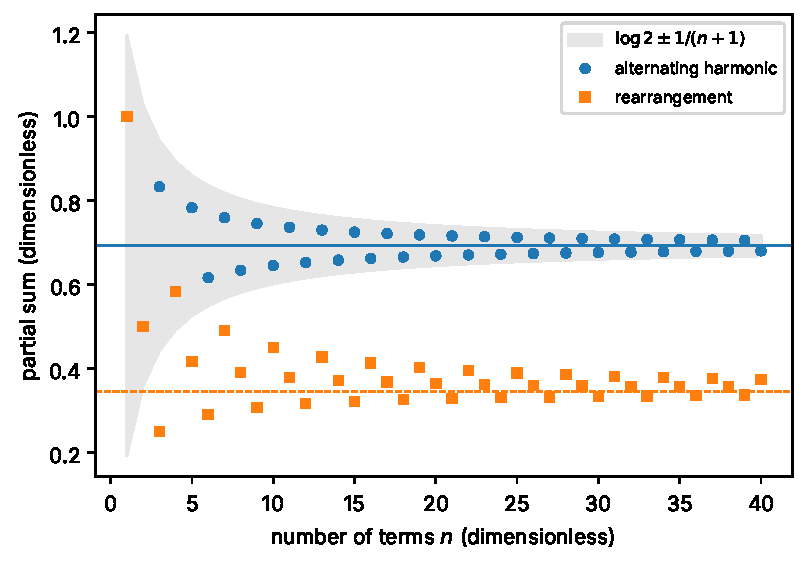
\includegraphics[width=0.85\linewidth]{figs/series_alternating.pdf}
\caption{Partial sums of the alternating harmonic series (circles), which zigzag around $\log 2$ with error at most the next term $1/(n+1)$ (shaded band), and of its rearrangement $1-\tfrac12-\tfrac14+\tfrac13-\tfrac16-\tfrac18+\cdots$ (squares), which uses exactly the same terms in a different order and converges to $\tfrac12\log2$.}
\label{fig:series-alternating}
\end{figure}

\begin{pitfall}
Never reorder, regroup in a way that changes which terms are paired, or ``sum by a different cutoff'' a series that is not absolutely convergent and expect the same answer. For an absolutely convergent series any order is fine (\cref{sec:series-absolute}); for a conditionally convergent one, the answer depends on the order. Sums over primes on the critical line are not absolutely convergent, so they fall outside the safe first kind (\cref{sec:series-truncation}).
\end{pitfall}

\begin{checkpoint}
You may rearrange $\sum(-1)^{k+1}/k^2$ freely, but not $\sum(-1)^{k+1}/k$. Why?
\end{checkpoint}
\checkanswer{The first converges absolutely, since $\sum1/k^2$ converges, so every rearrangement has the same sum. The second converges only conditionally, and we exhibited a rearrangement with half the sum.}

\begin{keyideas}
\item Alternating series with decreasing terms tending to zero converge, and the error is at most the first omitted term (Eq.~\eqref{eq:series-alt-error}).
\item The alternating harmonic series converges conditionally to $\log2$.
\item Rearranging a conditionally convergent series can change its sum: the order of summation matters.
\end{keyideas}

\section{The ratio test, power series and the logarithm series}\label{sec:series-power}

\subsection{The ratio test}

The geometric series is the yardstick for many others. If successive terms shrink by a factor eventually smaller than some fixed $r<1$, the series is dominated by a geometric one.

\textbf{Theorem (ratio test).} Suppose $a_k\ne0$ and $\abs{a_{k+1}/a_k}\to L$. If $L<1$ the series $\sum a_k$ converges absolutely; if $L>1$ it diverges; if $L=1$ the test gives no information.

\emph{Proof.} Case $L<1$: choose $r=(L+1)/2$, so $L<r<1$. Since the ratios tend to $L$, there is a $K$ with $\abs{a_{k+1}/a_k}<r$ for all $k\ge K$. Then $\abs{a_{K+1}}<r\abs{a_K}$, $\abs{a_{K+2}}<r\abs{a_{K+1}}<r^2\abs{a_K}$, and by induction $\abs{a_{K+j}}<r^j\abs{a_K}$. The series $\sum_j\abs{a_K}r^j$ is geometric with ratio $r<1$ and converges, so by comparison $\sum_{k\ge K}\abs{a_k}$ converges; the finitely many terms before $K$ do not matter.

Case $L>1$: there is a $K$ with $\abs{a_{k+1}/a_k}>1$ for $k\ge K$, so $\abs{a_k}\ge\abs{a_K}>0$ for all $k\ge K$. The terms do not tend to zero, and the series diverges.

Case $L=1$: for the $p$-series, $\abs{a_{k+1}/a_k}=(k/(k+1))^s\to1$ for every real $s$, yet the series converges for $s>1$ and diverges for $s\le1$. So $L=1$ decides nothing. $\square$

\subsection{Power series and the radius of convergence}

A \textbf{power series} in a variable $z$ (real or complex) is $\sum_{m=0}^\infty c_mz^m$. Applying the ratio test to $a_m=c_mz^m$,
\[
\left|\frac{c_{m+1}z^{m+1}}{c_mz^m}\right|=\abs z\left|\frac{c_{m+1}}{c_m}\right|.
\]
Assume all $c_m\ne0$. If $\abs{c_m/c_{m+1}}\to R$ with $0<R<\infty$, this ratio tends to $\abs z/R$. If $R=\infty$ the ratio tends to $0$ for every $z$. If $R=0$ it tends to infinity for every $z\ne0$, and the series converges only at $z=0$. So the series converges absolutely for $\abs z<R$ and diverges for $\abs z>R$. The number $R$ is the \textbf{radius of convergence}: in the complex plane the series converges inside the disk of radius $R$ and diverges outside it. On the circle $\abs z=R$ anything can happen and each point must be examined separately. (A radius of convergence exists for every power series, even when the ratio limit does not; we only need the ratio version.)

Examples:
\begin{itemize}
\item Geometric, $c_m=1$: $R=1$.
\item Exponential, $c_m=1/m!$ (Chapter~\ref{ch:complex}): $\abs{c_m/c_{m+1}}=(m+1)!/m!=m+1\to\infty$, so $R=\infty$; $e^z$ converges for every $z$.
\item $c_m=1/m$ ($m\ge1$): $\abs{c_m/c_{m+1}}=(m+1)/m\to1$, so $R=1$. This is the logarithm series, next.
\end{itemize}

\subsection{The series for $-\log(1-x)$}

We derive the Taylor series of $\log(1-x)$ with complete control of the error, starting from the finite geometric sum. For $u\ne1$, Eq.~\eqref{eq:series-geom-partial} says $\sum_{m=0}^{n-1}u^m=(1-u^n)/(1-u)$. Rearranged:
\[
\frac1{1-u}=\sum_{m=0}^{n-1}u^m+\frac{u^n}{1-u}.
\]
This is an exact identity, not an approximation. Integrate both sides over $u$ from $0$ to $x$, for real $x<1$ (so that $1-u>0$ throughout).

The left side: substitute $w=1-u$, $\dd w=-\dd u$, with $w$ running from $1$ to $1-x$:
\[
\int_0^x\frac{\dd u}{1-u}=-\int_1^{1-x}\frac{\dd w}{w}=-\log(1-x).
\]
On the right, $\int_0^xu^m\,\dd u=x^{m+1}/(m+1)$. Relabel $m+1\to m$ in the sum:
\begin{equation}
-\log(1-x)=\sum_{m=1}^{n}\frac{x^m}{m}+R_n(x),\qquad R_n(x)=\int_0^x\frac{u^n}{1-u}\,\dd u .
\label{eq:series-log-remainder}
\end{equation}
Now bound the remainder.

\emph{Case $0\le x<1$.} For $0\le u\le x$, $1-u\ge1-x>0$, so $0\le u^n/(1-u)\le u^n/(1-x)$, and
\[
0\le R_n(x)\le\frac1{1-x}\int_0^xu^n\,\dd u=\frac{x^{n+1}}{(n+1)(1-x)}\to0 .
\]
\emph{Case $-1\le x<0$.} Substitute $u=-v$ ($\dd u=-\dd v$; $v$ runs from $0$ to $\abs x$):
\[
R_n(x)=\int_0^{\abs x}\frac{(-v)^n}{1+v}(-\dd v)=(-1)^{n+1}\int_0^{\abs x}\frac{v^n}{1+v}\,\dd v .
\]
Since $1/(1+v)\le1$ for $v\ge0$, $\abs{R_n(x)}\le\int_0^{\abs x}v^n\,\dd v=\abs x^{n+1}/(n+1)\to0$, even at $x=-1$.

In both cases $R_n\to0$, so the partial sums converge to the left side:
\begin{equation}
-\log(1-x)=\sum_{m=1}^{\infty}\frac{x^m}{m}=x+\frac{x^2}2+\frac{x^3}3+\cdots\qquad(-1\le x<1).
\label{eq:series-log}
\end{equation}
At $x=-1$ this reads $-\log2=-1+\tfrac12-\tfrac13+\cdots$, that is,
\begin{equation}
\log2=1-\frac12+\frac13-\frac14+\cdots,
\label{eq:series-log2}
\end{equation}
the promised value of the alternating harmonic series. At $x=1$ both sides fail: $\log0$ is undefined and the harmonic series diverges. The radius of convergence is $1$, consistent with the ratio computation above. \Cref{fig:series-logseries} shows how the truncations approach $-\log(1-x)$ inside the interval and fail near $x=1$.

\begin{figure}[htbp]\centering
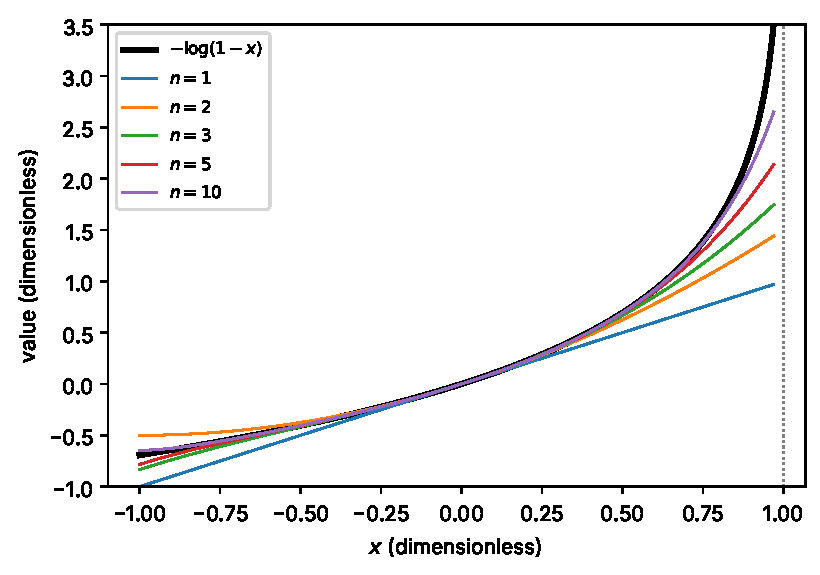
\includegraphics[width=0.85\linewidth]{figs/series_logseries.pdf}
\caption{The function $-\log(1-x)$ (thick line) and its truncations $\sum_{m=1}^nx^m/m$ for $n=1,2,3,5,10$. Near $x=0$ a few terms suffice; as $x\to1$ the function blows up while every truncation stays finite, so more and more terms are needed. The radius of convergence is 1.}
\label{fig:series-logseries}
\end{figure}

\begin{sample}{$\log 1.5$ from three terms}
Use Eq.~\eqref{eq:series-log-remainder} with three terms to approximate $\log1.5$ and bound the error.

\textbf{Step 1 (choose $x$):} $-\log(1-x)=\log\frac1{1-x}$. We want $\frac1{1-x}=1.5$, i.e. $1-x=\tfrac23$, $x=\tfrac13$.

\textbf{Step 2 (three terms):} $\tfrac13+\tfrac{(1/3)^2}2+\tfrac{(1/3)^3}3=0.333333+0.055556+0.012346=0.401235$.

\textbf{Step 3 (error bound, case $0\le x<1$, $n=3$):} $R_3\le\frac{x^4}{4(1-x)}=\frac{1/81}{4\cdot\frac23}=\frac{0.0123457}{2.666667}=0.004630$.

\textbf{Step 4 (compare):} The true value is $\log1.5=0.405465$; the actual error is $0.004230$, positive and below the bound, as the analysis predicts.

\[\boxed{\log1.5\approx0.401235,\quad 0<\text{error}\le0.00463}\]
\end{sample}

\subsection{Complex arguments}

For complex $z$ with $\abs z<1$, the series $\sum_{m\ge1}z^m/m$ converges absolutely, by comparison with the geometric series $\sum\abs z^m$ (since $\abs{z^m/m}\le\abs z^m$). What is it the logarithm of?

\begin{beyond}
\textbf{The complex logarithm series (proved; proof beyond this book).} For complex $z$ with $\abs z<1$, the sum $L(z)=\sum_{m=1}^\infty z^m/m$ satisfies $e^{L(z)}=\frac1{1-z}$. Thus $L(z)$ is a logarithm of $1/(1-z)$; it is the principal one (Chapter~\ref{ch:complex}), with imaginary part between $-\pi/2$ and $\pi/2$ because $1-z$ lies in the right half-plane. The proof differentiates the power series term by term, which is legitimate inside the radius of convergence; see Riley, Hobson and Bence~\cite{rhb}. A direct numerical computation, summing 200 terms at $z=\tfrac12e^{i}$, confirms the identity to within $10^{-12}$.
\end{beyond}

The case we will use again and again: $z=p^{-s}$ with $p$ a prime and $s=\sigma+it$. By Eq.~\eqref{eq:series-ks-modulus}, $\abs{p^{-s}}=p^{-\sigma}$, which is below 1 whenever $\sigma>0$. So
\[
-\log\bigl(1-p^{-s}\bigr)=\sum_{m=1}^\infty\frac{p^{-ms}}{m}\qquad(\Re s>0),
\]
with the series converging absolutely. This is the step that turns the Euler product into the explicit formula (Chapter~\ref{ch:explicit-formula}).

\subsection{Running example RE2: truncating the powers of a prime}

The prime-2 wave of the paper's continuation probe (RE2) is
\[
f_2(t)=-\frac1\pi\sum_{m=1}^{3}\frac{\sin(mt\log2)}{m\,2^{m/2}} .
\]
The explicit formula, before truncation in $m$, would contain all $m\ge1$. Call that version $f_2^{\infty}(t)$. Does it exist, and how much does stopping at $m=3$ change it?

\begin{sample}{How much is lost by keeping only $m\le3$?}
Show that $f_2^\infty(t)$ converges absolutely for every real $t$ and bound $\abs{f_2^\infty(t)-f_2(t)}$.

\textbf{Step 1 (absolute convergence):} $\abs{\sin(mt\log2)}\le1$, so the $m$-th term has modulus at most $\frac1\pi\frac{2^{-m/2}}m$. The series $\sum_m2^{-m/2}/m$ is Eq.~\eqref{eq:series-log} at $x=2^{-1/2}=0.707107<1$, so it converges. By comparison, $f_2^\infty(t)$ converges absolutely for every $t$.

\textbf{Step 2 (exact tail of the moduli):} By Eq.~\eqref{eq:series-log}, $\sum_{m=1}^\infty\frac{2^{-m/2}}m=-\log(1-2^{-1/2})=-\log0.292893=1.227947$. The first three terms are $0.707107+\frac{0.5}{2}+\frac{0.353553}{3}=0.707107+0.25+0.117851=1.074958$.

\textbf{Step 3 (bound):} By Eq.~\eqref{eq:series-abs-ineq} applied to the tail,
\[
\abs{f_2^\infty(t)-f_2(t)}\le\frac1\pi\sum_{m=4}^\infty\frac{2^{-m/2}}m=\frac{1.227947-1.074958}{\pi}=\frac{0.152989}{\pi}.
\]

\textbf{Step 4 (an alternative, cruder bound, for comparison):} Using $1/m\le1/4$ for $m\ge4$ and Eq.~\eqref{eq:series-geom-sum}: $\frac1{4\pi}\sum_{m\ge4}2^{-m/2}=\frac1{4\pi}\frac{2^{-2}}{1-2^{-1/2}}=0.067924$. This is also a valid upper bound, but it is larger than the Step~3 value $0.152989/\pi=0.048698$, so the Step~3 bound is the tighter one and is the one we keep.

\begin{equation}
\boxed{\abs{f_2^\infty(t)-f_2(t)}\le0.048698\ \text{ for all } t}
\label{eq:series-re2-tail}
\end{equation}
For scale: the amplitude of the leading term is $2^{-1/2}/\pi=0.225079$. The neglected powers can shift the wave by at most about a fifth of its leading amplitude ($0.0487/0.2251=0.216$), and that worst case requires all neglected sines to peak together. \Cref{fig:series-re2} compares the truncations.
\end{sample}

\begin{figure}[htbp]\centering
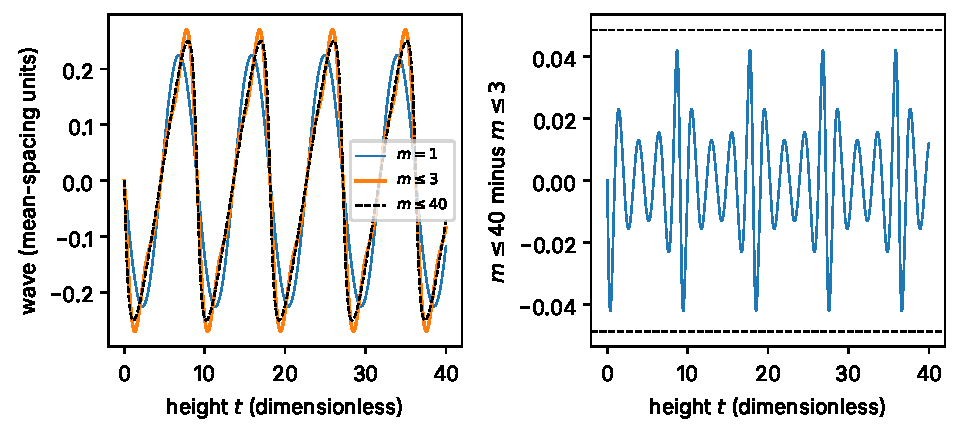
\includegraphics[width=0.85\linewidth]{figs/series_re2.pdf}
\caption{Running example RE2. Left: the prime-2 wave $-\frac1\pi\sum_m\sin(mt\log2)/(m2^{m/2})$ truncated at $m=1$, at $m\le3$ (the paper's choice), and at $m\le40$ (effectively the full absolutely convergent series), for $0\le t\le40$. The pattern repeats with period $2\pi/\log2\approx9.065$. Right: the difference between the $m\le40$ and $m\le3$ versions stays inside the guaranteed bound $\pm0.0487$ of Eq.~\eqref{eq:series-re2-tail} (dashed).}
\label{fig:series-re2}
\end{figure}

\begin{checkpoint}
For which real $x$ does $\sum_{m=1}^\infty x^m/m$ converge? For which complex $z$ does it converge absolutely?
\end{checkpoint}
\checkanswer{For real $x$: exactly $-1\le x<1$ (diverges at $x=1$ as the harmonic series, diverges for $\abs x>1$ by the ratio test). It converges absolutely for complex $\abs z<1$; at $x=-1$ it converges only conditionally.}

\begin{keyideas}
\item Ratio test: $\abs{a_{k+1}/a_k}\to L<1$ gives absolute convergence, $L>1$ divergence, $L=1$ no information.
\item A power series converges absolutely inside its radius of convergence $R=\lim\abs{c_m/c_{m+1}}$ and diverges outside.
\item $-\log(1-x)=\sum_{m\ge1}x^m/m$ for $-1\le x<1$, derived with an explicit remainder (Eqs.~\eqref{eq:series-log-remainder}, \eqref{eq:series-log}); at $x=-1$ it gives $\log2$.
\item For $\abs z<1$ the same series is the principal logarithm of $1/(1-z)$; in particular $-\log(1-p^{-s})=\sum_m p^{-ms}/m$ for $\Re s>0$.
\item Truncating the prime-2 wave at $m\le3$ changes it by at most $0.0487$ (Eq.~\eqref{eq:series-re2-tail}).
\end{keyideas}

\section{Infinite products}\label{sec:series-products}

\subsection{Definition}

An \textbf{infinite product} $\prod_{k=1}^\infty u_k=u_1u_2u_3\cdots$ is defined, like a series, through its partial products
\begin{equation}
P_n=\prod_{k=1}^nu_k=u_1u_2\cdots u_n .
\label{eq:series-prod-def}
\end{equation}
\textbf{Definition.} The product \textbf{converges} if $P_n\to P$ with $P$ a finite number \emph{different from zero}. If $P_n\to0$ while no factor is zero, we say the product \textbf{diverges to zero}.

Why exclude zero? Two reasons. First, for a finite product, $P=0$ happens only if some factor is zero; we want the same for convergent infinite products, so that a product formula for a function tells us where it vanishes (this is how Chapter~\ref{ch:zeta} proves that $\zeta(s)\ne0$ for $\Re s>1$). Second, we want logarithms to turn convergent products into convergent sums, and $\log 0$ does not exist.

Writing $u_k=1+a_k$, a convergent product must have $a_k\to0$: indeed $u_n=P_n/P_{n-1}\to P/P=1$ (the division is allowed because $P\ne0$). This is the product version of the term test.

\subsection{Three telescoping examples}

\emph{(i) Diverges to infinity.} $\prod_{k=1}^n\left(1+\frac1k\right)=\prod_{k=1}^n\frac{k+1}{k}=\frac21\cdot\frac32\cdots\frac{n+1}{n}=n+1\to\infty$. (Each numerator cancels the next denominator.)

\emph{(ii) Diverges to zero.} $\prod_{k=2}^n\left(1-\frac1k\right)=\prod_{k=2}^n\frac{k-1}k=\frac12\cdot\frac23\cdots\frac{n-1}n=\frac1n\to0$. No factor is zero, yet the partial products vanish in the limit. By our definition this product diverges.

\emph{(iii) Converges.} See the Sample Problem.

\begin{sample}{A product that converges to one half}
Evaluate $\prod_{k=2}^n\left(1-\frac1{k^2}\right)$ and its limit.

\textbf{Step 1 (factor):} $1-\frac1{k^2}=\frac{k^2-1}{k^2}=\frac{(k-1)(k+1)}{k\cdot k}=\frac{k-1}k\cdot\frac{k+1}k$.

\textbf{Step 2 (split the product):} $\prod_{k=2}^n\left(1-\frac1{k^2}\right)=\left[\prod_{k=2}^n\frac{k-1}k\right]\left[\prod_{k=2}^n\frac{k+1}k\right]$ (finite products may be reordered).

\textbf{Step 3 (telescope each):} The first is $\frac1n$ (example (ii)). The second is $\frac32\cdot\frac43\cdots\frac{n+1}n=\frac{n+1}2$.

\textbf{Step 4:} So $P_n=\frac1n\cdot\frac{n+1}2=\frac{n+1}{2n}\to\frac12$. At $n=10$, $P_{10}=\frac{11}{20}=0.55$.

\[\boxed{\prod_{k=2}^\infty\left(1-\frac1{k^2}\right)=\frac12}\]
Notice that the two pieces individually diverge (to $0$ and to $\infty$), but their product converges. Splitting an infinite product into divergent pieces is dangerous; here we split only the \emph{finite} partial products, which is always safe.
\end{sample}

\subsection{From products to sums: the logarithm}

For a finite product of positive numbers, $\log(u_1u_2\cdots u_n)=\log u_1+\log u_2+\cdots+\log u_n$ (apply $\log(ab)=\log a+\log b$ repeatedly). The infinite version:

\textbf{Theorem.} Let $u_k>0$. The product $\prod u_k$ converges (to a positive $P$) if and only if the series $\sum\log u_k$ converges, and then
\begin{equation}
\log\prod_{k=1}^\infty u_k=\sum_{k=1}^\infty\log u_k .
\label{eq:series-prod-log}
\end{equation}
The product diverges to zero exactly when $\sum_{k\le n}\log u_k\to-\infty$.

\emph{Proof.} Let $L_n=\sum_{k=1}^n\log u_k=\log P_n$, so $P_n=e^{L_n}$. If $L_n\to L$, then $P_n=e^{L_n}\to e^{L}>0$ because $e^x$ is continuous; so the product converges to $e^L$ and $\log P=L$. Conversely, if $P_n\to P>0$, then $L_n=\log P_n\to\log P$ because $\log$ is continuous at the positive number $P$. Finally $P_n=e^{L_n}\to0$ if and only if $L_n\to-\infty$. $\square$

Example (ii) in this language: $\sum_{k=2}^n\log(1-1/k)=\log(1/n)=-\log n\to-\infty$.

\begin{pitfall}
For complex numbers, $\log(zw)=\log z+\log w$ can fail for the principal logarithm, because the arguments may add up beyond $\pi$ and the principal value wraps around (Chapter~\ref{ch:complex}). Example: $z=w=e^{2\pi i/3}$. Principal values: $\log z+\log w=\tfrac{4\pi i}3$, but $zw=e^{4\pi i/3}=e^{-2\pi i/3}$ has principal logarithm $-\tfrac{2\pi i}3$. They differ by $2\pi i$. Eq.~\eqref{eq:series-prod-log} is safe as stated for positive factors; for complex factors one must keep track of the branch, a point Chapter~\ref{ch:explicit-formula} handles when it takes $\log\zeta(s)$.
\end{pitfall}

\subsection{When does $\prod(1+a_k)$ converge?}

\textbf{Theorem.} Let $a_k\ge0$. Then $\prod_{k=1}^\infty(1+a_k)$ converges if and only if $\sum_{k=1}^\infty a_k$ converges. Moreover, with $A=\sum a_k$,
\begin{equation}
1+A\le\prod_{k=1}^\infty(1+a_k)\le e^{A}.
\label{eq:series-prod-bounds}
\end{equation}

\emph{Proof.} Each factor is at least $1$, so the partial products $P_n$ increase. Let $A_n=\sum_{k=1}^na_k$.

\emph{Upper bound.} For $a\ge0$, $1+a\le e^a$: the function $g(a)=e^a-1-a$ has $g(0)=0$ and $g'(a)=e^a-1\ge0$ for $a\ge0$, so $g(a)\ge0$. Multiplying these inequalities (all quantities positive), $P_n\le e^{a_1}\cdots e^{a_n}=e^{A_n}$.

\emph{Lower bound.} $P_n\ge1+A_n$, by induction: $P_1=1+a_1$; if $P_n\ge1+A_n$ then
\[
P_{n+1}=P_n(1+a_{n+1})\ge(1+A_n)(1+a_{n+1})=1+A_n+a_{n+1}+A_na_{n+1}\ge1+A_{n+1},
\]
since $A_na_{n+1}\ge0$.

If $\sum a_k$ converges, $P_n\le e^{A_n}\le e^{A}$: increasing and bounded, so $P_n$ converges to a limit at least $P_1\ge1$, hence nonzero. If $\sum a_k$ diverges, $P_n\ge1+A_n\to\infty$. Taking $n\to\infty$ in the two bounds gives Eq.~\eqref{eq:series-prod-bounds}. $\square$

Example (i) is the divergent case: $a_k=1/k$, harmonic. By contrast $\prod(1+1/k^2)$ converges, and Eq.~\eqref{eq:series-prod-bounds} brackets it between $1+\pi^2/6$ and $e^{\pi^2/6}$ (Problem~13).

\begin{beyond}
\textbf{Complex factors (proved; proof beyond this book).} If $a_k$ are complex and $\sum\abs{a_k}$ converges, then $\prod(1+a_k)$ converges in the sense above unless some factor $1+a_k$ is exactly zero; in that case the limit is $0$, and only then. Such a product can also be rearranged without changing its value. Proofs are in Apostol~\cite{apostol}, in the chapter on Euler products, and in Titchmarsh~\cite{titchmarsh}.
\end{beyond}

\subsection{A first look at the Euler product}

List the primes in increasing order, $p_1=2,\ p_2=3,\ p_3=5,\dots$ (Chapter~\ref{ch:primes}). For real $s>1$ consider
\begin{equation}
\prod_{p}\frac1{1-p^{-s}}=\frac1{1-2^{-s}}\cdot\frac1{1-3^{-s}}\cdot\frac1{1-5^{-s}}\cdots
\label{eq:series-euler-preview}
\end{equation}
\emph{It converges.} Write each factor as $1+a_p$:
\[
\frac1{1-p^{-s}}=\frac{p^s}{p^s-1}=1+\frac{1}{p^s-1},\qquad a_p=\frac1{p^s-1}>0 .
\]
Since $p\ge2$ and $s>1$, $p^s>2$, so $p^s/2>1$ and therefore $p^s-1>p^s-p^s/2=p^s/2$. Hence $a_p<2p^{-s}$. The sum $\sum_p p^{-s}$ over primes is at most $\sum_k k^{-s}=\zeta(s)$ over all integers (its terms are a subset of nonnegative terms), so it converges; by comparison $\sum_pa_p$ converges, and by the theorem the product converges to a number at least 1.

Euler discovered that its value is $\zeta(s)$. The proof needs the unique factorization of integers into primes (Chapter~\ref{ch:primes}) and is given in Chapter~\ref{ch:zeta}; here we only look at the numbers for $s=2$, where $\zeta(2)=\pi^2/6=1.644934$. Each factor is $\frac1{1-p^{-2}}=\frac{p^2}{p^2-1}$: $\frac43,\ \frac98,\ \frac{25}{24},\ \frac{49}{48},\ \frac{121}{120},\ \frac{169}{168},\dots$

\begin{sample}{The Euler product at $s=2$ over primes up to 13}
Write $\Pi(x)=\prod_{p\le x}p^2/(p^2-1)$ for the partial Euler product over the primes up to $x$. Compute $\Pi(x)$ for $x=2,3,5,7,11,13$ and compare each value with $\pi^2/6$.

\textbf{Step 1:} $\Pi(2)=\frac43=1.333333$.

\textbf{Step 2:} $\Pi(3)=\frac43\cdot\frac98=\frac{36}{24}=1.5$.

\textbf{Step 3:} $\Pi(5)=1.5\cdot\frac{25}{24}=\frac{25}{16}=1.5625$.

\textbf{Step 4:} $\Pi(7)=\frac{25}{16}\cdot\frac{49}{48}=\frac{1225}{768}=1.595052$.

\textbf{Step 5:} $\Pi(11)=1.595052\cdot\frac{121}{120}=1.608344$; $\Pi(13)=1.608344\cdot\frac{169}{168}=1.617918$.

\textbf{Step 6:} Divide by $\pi^2/6$ (\cref{tab:series-euler}).

\[\boxed{\prod_{p\le13}\frac{p^2}{p^2-1}=1.617918=0.9836\times\frac{\pi^2}{6}}\]
Six primes already give 98.4\% of $\zeta(2)$. \Cref{fig:series-products} (right) continues to 100 primes.
\end{sample}

\begin{table}[htbp]\centering
\caption{Partial Euler products $\Pi(x)=\prod_{p\le x}(1-p^{-2})^{-1}$ and their ratio to $\zeta(2)=\pi^2/6=1.644934$.}
\label{tab:series-euler}
\begin{tabular}{ccc}
\toprule
largest prime $x$ & partial product $\Pi(x)$ & ratio to $\pi^2/6$\\
\midrule
2 & 1.333333 & 0.8106\\
3 & 1.500000 & 0.9119\\
5 & 1.562500 & 0.9499\\
7 & 1.595052 & 0.9697\\
11 & 1.608344 & 0.9778\\
13 & 1.617918 & 0.9836\\
\bottomrule
\end{tabular}
\end{table}

\begin{figure}[htbp]\centering
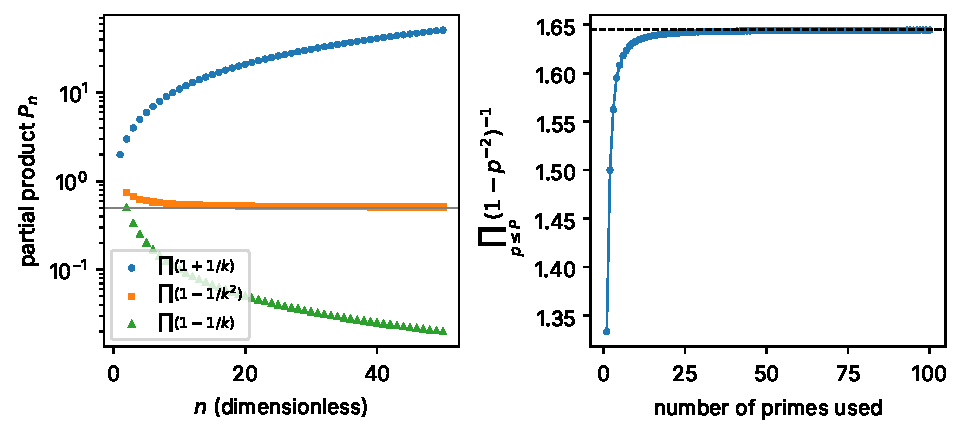
\includegraphics[width=0.85\linewidth]{figs/series_products.pdf}
\caption{Left: partial products of $\prod(1+1/k)$ (grows like $n+1$), $\prod(1-1/k^2)$ (converges to $\tfrac12$) and $\prod(1-1/k)$ (diverges to zero like $1/n$), for $n$ up to 50, on a logarithmic vertical axis. Right: the partial Euler product $\prod_{p\le x}(1-p^{-2})^{-1}$ against the number of primes used, approaching $\zeta(2)=\pi^2/6$ (dashed line).}
\label{fig:series-products}
\end{figure}

Taking the logarithm of the partial Euler product and expanding each factor with Eq.~\eqref{eq:series-log}, using $p^{-s}$ (which lies in $(0,\tfrac12]$) in place of the variable of that equation:
\[
\log\prod_{p\le x}\frac1{1-p^{-s}}=\sum_{p\le x}-\log(1-p^{-s})=\sum_{p\le x}\sum_{m=1}^\infty\frac{p^{-ms}}{m}.
\]
Letting $x\to\infty$ produces a \emph{double series} over primes $p$ and powers $m$. All its terms are positive here, so we may sum them in any order; the precise statement is in the box below. Chapter~\ref{ch:explicit-formula} repeats this computation for complex $s$ and then moves toward the critical line, where this freedom is lost.

\begin{beyond}
\textbf{Double series (proved; proof beyond this book).} If $b_{pm}\ge0$, or more generally if $\sum_p\sum_m\abs{b_{pm}}<\infty$, then the double series $\sum_{p,m}b_{pm}$ has the same value whether you sum over $m$ first, over $p$ first, or along any enumeration of the pairs $(p,m)$. The proof extends the rearrangement argument of \cref{sec:series-absolute}; see Apostol~\cite{apostol} or Riley, Hobson and Bence~\cite{rhb}.
\end{beyond}

\begin{checkpoint}
The partial products of $\prod_{k\ge2}(1-1/k)$ tend to a limit. Does the product converge?
\end{checkpoint}
\checkanswer{No. The limit is $0$ while no factor is zero, so by definition the product diverges to zero. Equivalently, $\sum\log(1-1/k)=-\infty$.}

\begin{keyideas}
\item An infinite product converges if its partial products tend to a finite \emph{nonzero} limit (Eq.~\eqref{eq:series-prod-def}); a convergent product needs factors tending to 1.
\item For positive factors, $\log\prod u_k=\sum\log u_k$, and the product converges iff the sum of logs does (Eq.~\eqref{eq:series-prod-log}).
\item For $a_k\ge0$: $\prod(1+a_k)$ converges iff $\sum a_k$ does, and $1+A\le\prod\le e^A$ (Eq.~\eqref{eq:series-prod-bounds}).
\item The Euler product $\prod_p(1-p^{-s})^{-1}$ converges for real $s>1$; numerically it approaches $\zeta(2)$ at $s=2$ (\cref{tab:series-euler}).
\end{keyideas}

\section{Truncation: when is a finite sum a good stand-in?}\label{sec:series-truncation}
% DYK-BEGIN
\begin{didyouknow}{The Slowest Infinity}
The harmonic series $1+\tfrac12+\tfrac13+\cdots$ diverges, as Nicole Oresme showed in the fourteenth century by grouping its terms. But it diverges incredibly slowly, because its partial sums grow like $\log N+0.5772\ldots$. To pass 100 you need roughly $1.5\times10^{43}$ terms. A truncated sum can look convergent long before it reveals its true nature.
\end{didyouknow}
% DYK-END

Every numerical use of an infinite series is a truncation. We now collect what the chapter has taught about the error of truncating, because the distinction matters for the paper.

\paragraph{Case 1: absolutely convergent series.} The truncation error is bounded by the tail of the moduli, $\abs{S-S_n}\le\sum_{k>n}\abs{a_k}$ (Eq.~\eqref{eq:series-abs-ineq}). That tail can be bounded in advance by a geometric series (Eq.~\eqref{eq:series-geom-tail}) or an integral (Eq.~\eqref{eq:series-tail-bounds}). The order of the terms does not matter. You know, before computing anything, how many terms you need. Examples: $\zeta(s)$ for $\Re s>1$ (Eq.~\eqref{eq:series-zeta-tail}); the sum over $m$ for one prime on the critical line (Eq.~\eqref{eq:series-re2-tail}).

\paragraph{Case 2: conditionally convergent series.} The sum exists but depends on the order of the terms (\cref{sec:series-alternating}). A truncation is meaningful only together with the order in which terms are added. For alternating series there is still an error bound (Eq.~\eqref{eq:series-alt-error}), but it is a special structure, not a general guarantee.

\paragraph{Case 3: divergent series.} The ``infinite sum'' does not exist, and adding more terms need not improve anything. Example: $\sum k^{-s}$ on the critical line (\cref{fig:series-spiral}). A finite piece of such a series can still be useful, but only if some \emph{other} argument says so: a smoothing that makes the sum converge, a rigorous theorem about a modified version, or numerical evidence. Until such an argument is supplied, the truncation is a heuristic.

\begin{table}[htbp]\centering
\caption{Three kinds of infinite sums and what truncation means for each.}
\label{tab:series-truncation}
\begin{tabular}{llll}
\toprule
kind & example & tail bound? & order matters?\\
\midrule
absolutely convergent & $\sum k^{-2-it}$ & yes, from moduli & no\\
conditionally convergent & $\sum(-1)^{k+1}/k$ & only special cases & yes\\
divergent & $\sum k^{-1/2-it}$ & no sum to approach & meaningless\\
\bottomrule
\end{tabular}
\end{table}

\paragraph{The sum over primes on the critical line.} The explicit formula (Chapter~\ref{ch:explicit-formula}) contains, on the line $s=\tfrac12+it$, the double sum
\[
-\frac1\pi\sum_p\sum_{m=1}^\infty\frac{\sin(mt\log p)}{m\,p^{m/2}} .
\]
Which case is it? Look at the sum of moduli bounds, power by power.
\begin{itemize}
\item $m\ge3$: the moduli are at most $\frac{p^{-m/2}}{m\pi}$, and their total over all primes and all $m\ge3$ is finite (Problem~27 bounds it by $0.584$). This part is absolutely convergent: Case 1.
\item $m=1$ and $m=2$: the moduli are at most the \emph{amplitudes} $\frac{p^{-1/2}}{\pi}$ and $\frac{p^{-1}}{2\pi}$ (we drop the factor $\abs{\sin(mt\log p)}\le1$). The sums of these amplitudes over primes diverge (first box below). So the comparison argument that worked for $m\ge3$ gives no tail bound here. In fact, for $t\ne0$ the sum of the actual moduli, $\frac1\pi\sum_p\abs{\sin(t\log p)}\,p^{-1/2}$, also diverges, because $\abs{\sin(t\log p)}$ is not small for most primes. Proving this needs the distribution of the primes, so we take it on trust in the second box below. Hence for $t\ne0$ the double sum is not absolutely convergent. Whether, and in what order of summation, it converges at all on the critical line is not something the tools of this chapter can settle; Chapter~\ref{ch:explicit-formula} treats it as a formal, heuristic object. What we can say is that for $t\ne0$ it is not absolutely convergent, so truncating it to a finite prime set comes with no tail bound from moduli, and it must be handled like Case 3: a truncation justified only by a separate argument.
\end{itemize}

\begin{beyond}
\textbf{The sum of reciprocals of the primes diverges (proved; proof beyond this chapter).} $\sum_p\frac1p=\frac12+\frac13+\frac15+\frac17+\cdots=\infty$. This is due to Euler; a proof, and the finer statement that $\sum_{p\le x}1/p$ equals $\log\log x$ plus a quantity that stays bounded as $x\to\infty$, is in Hardy and Wright~\cite{hardywright} and Apostol~\cite{apostol}. Since $p^{-1/2}\ge p^{-1}$, it follows by comparison that $\sum_pp^{-1/2}$ diverges as well.
\end{beyond}

\begin{beyond}
\textbf{The actual moduli also have infinite sum (proved; proof beyond this book).} For every real $t\ne0$, $\sum_p\abs{\sin(t\log p)}\,p^{-1/2}=\infty$, and likewise $\sum_p\abs{\sin(2t\log p)}\,p^{-1}=\infty$. The idea is that the angles $t\log p$ are spread around the circle, so a fixed fraction of the primes have $\abs{\sin(t\log p)}$ bounded away from zero. Making this precise uses the prime number theorem (Chapter~\ref{ch:primes}) in a form that controls oscillating sums over primes; see Davenport~\cite{davenport} or Titchmarsh~\cite{titchmarsh} for the tools. At $t=0$ every term vanishes, which is why the restriction $t\ne0$ is needed.
\end{beyond}

That the truncated prime sum nevertheless predicts the zeros remarkably well is a fact, but it is established in the paper by numerical tests, and in the literature by rigorous theorems about smoothed versions of the formula (Chapter~\ref{ch:explicit-formula}), not by the convergence theory of this chapter.

\begin{keyideas}
\item Truncation error is under control in advance only for absolutely convergent series (\cref{tab:series-truncation}).
\item In the critical-line prime sum, the $m\ge3$ part converges absolutely. For $m=1$ and $m=2$ the amplitude sums diverge (because $\sum_p1/p$ does), so comparison gives no tail bound. For $t\ne0$ the actual moduli also have infinite sum (taken on trust), so these parts are not absolutely convergent.
\item A finite piece of a non-absolutely-convergent sum needs a separate justification: a theorem about a modified sum or numerical evidence.
\end{keyideas}

\section{Paper connection}\label{sec:series-paper}

Here is where this chapter's tools meet the paper~\cite{soniR1}, revision R1.

\paragraph{The zeros cannot be computed by summing the defining series (Sec.~II~A).} The paper writes the zeros as $\rho_n=\tfrac12+it_n$ and records $t_1=14.134725141734695$. At $s=\rho_n$ the Dirichlet series $\sum k^{-s}$ is not absolutely convergent and in fact diverges (\cref{sec:series-absolute}, \cref{fig:series-spiral}). So the statement ``$\zeta(\rho_n)=0$'' refers to the analytically continued function of Chapter~\ref{ch:zeta}, and the zeros themselves are computed by specialized methods (\texttt{mpmath.zetazero}, App.~A step~1), not by adding terms of $\sum k^{-s}$.

\paragraph{Eq.~(4) is a finite double sum.} The arithmetic oracle of the paper (Sec.~II~D, Eq.~(4)) is
\[
N_{\rm fl}(t)=-\frac1\pi\sum_{p\in P}\sum_{m=1}^{3}\frac{\sin(mt\log p)}{m\,p^{m/2}},
\]
a sum of $3\abs P$ sinusoids. It is truncated in two ways.
\begin{itemize}
\item \emph{In $m$:} App.~A step~8 states $m\le3$. For each prime the full $m$-series converges absolutely on the critical line, and Eq.~\eqref{eq:series-re2-tail} bounds what is dropped: at most $0.0487$ for $p=2$, and at most $0.0169$ for $p=3$ (Problem~15). These bounds are theorems.
\item \emph{In $p$:} the prime set $P$ is finite (one prime, 3, 6 or 25 primes in Table~V; 300 primes, ``900 terms'', in row A of Table~IV). The full sum over all primes is not absolutely convergent for $t\ne0$ (\cref{sec:series-truncation}), so there is no tail bound from this chapter and the effect of adding primes is a matter of evidence.
\end{itemize}

\paragraph{The evidence (Table~V and Table~IV).} On the principal holdout, zeros 401--500 (running example RE5, null rms $0.263$), Table~V reports rms errors (in mean spacings) of $0.198$ with $\{2\}$, $0.116$ with 3 primes, $0.074$ with 6 primes and $0.043$ with 25 primes, with correlations $+0.66$, $+0.90$, $+0.96$, $+0.99$. Table~IV, row A, gives $0.018$ with 300 primes, and Sec.~IV states that the oracle ``improves monotonically'' as the budget grows. Read with this chapter's eyes, these are \emph{numerical observations} about a truncation of a non-absolutely-convergent sum. They show that the truncated sum is useful at these heights; they are not a proof that the sum converges, and the paper does not claim one (it calls Eq.~(4) a truncation with ``no novelty'' and attributes its theory to Refs.~\cite{francaleclair,leclair}). You can reproduce the Table~V row yourself:

\begin{pycode}
import numpy as np, qmnt
n = np.arange(401, 501)                    # holdout RE5
# the null predicts zero fluctuation, so its corr is undefined (nan)
print("null", qmnt.score(qmnt.smooth_zeros(n), n))
for k in [1, 3, 6, 25]:                    # prime budgets of Table V
    P = qmnt.first_primes(k)
    tp = qmnt.oracle_zeros(n, P, mmax=3)   # solve Nsm + Nfl = n - 1/2
    rms, corr = qmnt.score(tp, n)
    print(k, round(rms, 3), round(corr, 2))
\end{pycode}

\paragraph{The continuation probe uses the RE2 wave (Sec.~III, App.~A step~15).} The paper's arithmetic-continuation probe replaces the true targets by the $p=2$, $m\le3$ part of Eq.~(4), which is exactly $f_2(t)$ of \cref{sec:series-power}, a finite sum of three sinusoids with period $2\pi/\log2\approx9.065$. Our bound Eq.~\eqref{eq:series-re2-tail} tells you that choosing $m\le3$ rather than all $m$ changes this target by at most $0.0487$ at any height. So a probe built from the full $m$-series would have used a target differing from the paper's by at most $0.0487$. The choice $m\le3$ is therefore immaterial to what the probe tests (in-sample rms $0.056$, held-out correlation $+0.07$), namely whether the fit can continue an oscillation at all (Chapter~\ref{ch:fourier-series}).

\paragraph{The state sum of Eq.~(5) is a truncated sum (Sec.~II~E).} The second-order shift in Eq.~(5),
\[
\delta E_n=-\sum_{m\ne n}\frac{\abs{A_{nm}}^2}{E_n-E_m},
\]
runs over unperturbed states $m$ (here $m$ labels states, not prime powers; $A$ is the non-Hermitian operator of Chapter~\ref{ch:non-hermitian}. It is not the sum $A=\sum a_k$ of \cref{sec:series-products}, nor the sensitivity matrix $A_{nk}$ of the paper's Sec.~II~C; the paper overloads the letter.). The paper sums ``over all 652 basis states with $E\le1000$'' and notes that ``truncating at 500 states measurably biases the top levels''. A plausible reading (ours, not the paper's): if the matrix elements $\abs{A_{nm}}^2$ of nearby states are of comparable size, the terms are largest when $E_m$ is close to $E_n$, so for the top levels the first omitted states are close in energy and contribute terms that are not small. A truncation is only as good as the size of what it leaves out, and for the top levels the leftover is not negligible. Chapters~\ref{ch:perturbation} and~\ref{ch:non-hermitian} develop the formula.

\paragraph{The sum rule rests on reordering a finite double sum (Sec.~V and Sec.~V~A).} Sec.~V~A states that $\sum_n\delta E_n=0$ ``exactly when summed over a complete truncated basis, since the contribution of each pair $(n,m)$ is antisymmetric''. Here is the general fact. Let $b_{nm}$ be numbers, for $n,m$ in a finite index set, with $b_{mn}=-b_{nm}$. Let
\begin{equation}
T=\sum_n\sum_{m\ne n}b_{nm}.
\label{eq:series-pair}
\end{equation}
Rename the summation letters ($n\leftrightarrow m$); this changes nothing, so $T=\sum_m\sum_{n\ne m}b_{mn}$. A finite double sum may be summed in either order, so $T=\sum_n\sum_{m\ne n}b_{mn}=\sum_n\sum_{m\ne n}(-b_{nm})=-T$. Hence $T=0$. With $b_{nm}=-\abs{A_{nm}}^2/(E_n-E_m)$, antisymmetry holds because swapping $n$ and $m$ flips the sign of the denominator and leaves $\abs{A_{nm}}^2=\abs{A_{mn}}^2$ unchanged (true for a real multiplication operator, as Chapter~\ref{ch:non-hermitian} shows). The word ``complete'' matters: if the sum over $m$ is cut off for some $n$ but the partner terms are kept for others, pairs are broken and the cancellation fails; for an infinite basis, the reordering step would additionally need absolute convergence (\cref{sec:series-absolute}). The paper reports the sum verified to $4\times10^{-15}$ in Sec.~V, and to $3.6\times10^{-15}$ (odd class) and $1.4\times10^{-14}$ (even class) in Sec.~V~A: zero up to floating-point round-off (Chapter~\ref{ch:asymptotics}).

\section{Summary}

\begin{itemize}
\item A sequence converges to $a$ if its terms eventually stay within any tolerance of $a$ (Eq.~\eqref{eq:series-limit-def}); $r^n\to0$ for $\abs r<1$; complex sequences converge iff real and imaginary parts do. Monotone bounded sequences converge (taken on trust).
\item A series converges when its partial sums converge; terms tending to zero is necessary, not sufficient.
\item Geometric series: $\sum_{k=0}^{n-1}r^k=(1-r^n)/(1-r)$; sum $1/(1-r)$ and tail $r^n/(1-r)$ for $\abs r<1$ (Eqs.~\eqref{eq:series-geom-partial}--\eqref{eq:series-geom-tail}).
\item Telescoping: $\sum_{k=1}^n(b_k-b_{k+1})=b_1-b_{n+1}$ (Eq.~\eqref{eq:series-telescope}).
\item The harmonic series diverges (Eq.~\eqref{eq:series-oresme}); $\log(n+1)\le H_n\le1+\log n$ and $H_n-\log n\to\gamma$ (Eqs.~\eqref{eq:series-harmonic-bounds}, \eqref{eq:series-gamma}).
\item Comparison and integral tests for nonnegative series; integral bounds on tails (Eqs.~\eqref{eq:series-integral-test}, \eqref{eq:series-tail-bounds}); $\sum k^{-s}$ converges iff $s>1$ (Eq.~\eqref{eq:series-pseries}).
\item Absolute convergence implies convergence, $\abs{\sum a_k}\le\sum\abs{a_k}$, and free rearrangement (Eq.~\eqref{eq:series-abs-ineq}). Since $\abs{k^{-s}}=k^{-\sigma}$ (Eq.~\eqref{eq:series-ks-modulus}), $\sum k^{-s}$ converges absolutely for $\Re s>1$ with tail at most $n^{1-\sigma}/(\sigma-1)$ (Eq.~\eqref{eq:series-zeta-tail}); it diverges on the critical line.
\item Alternating series converge with error at most the first omitted term (Eq.~\eqref{eq:series-alt-error}); conditionally convergent series can change their sum under rearrangement.
\item Ratio test; radius of convergence; $-\log(1-x)=\sum x^m/m$ for $-1\le x<1$ with explicit remainder, giving $\log2$ (Eqs.~\eqref{eq:series-log-remainder}--\eqref{eq:series-log2}); $-\log(1-p^{-s})=\sum_mp^{-ms}/m$ for $\Re s>0$.
\item Truncating the prime-2 wave at $m\le3$ costs at most $0.0487$ (Eq.~\eqref{eq:series-re2-tail}).
\item Infinite products converge to nonzero limits; logs turn them into sums (Eqs.~\eqref{eq:series-prod-def}, \eqref{eq:series-prod-log}); $\prod(1+a_k)$ with $a_k\ge0$ converges iff $\sum a_k$ does, with $1+A\le\prod\le e^A$ (Eq.~\eqref{eq:series-prod-bounds}); the Euler product converges for $s>1$ (Eq.~\eqref{eq:series-euler-preview}).
\item Truncations have controlled error only for absolutely convergent series (\cref{tab:series-truncation}); the critical-line prime sum is not absolutely convergent for $t\ne0$ (its $m=1,2$ amplitude sums diverge, and, as taken on trust, so do its actual moduli), so the success of Eq.~(4) of the paper is a numerical observation.
\item Antisymmetric pair contributions cancel in a finite double sum (Eq.~\eqref{eq:series-pair}), the basis of the paper's sum rule.
\end{itemize}

\section{Problems}

\begin{problemlist}
\prob{1}{Compute the partial sum $S_4=\sum_{k=0}^{3}(1/3)^k$ as a fraction, and the sum $\sum_{k=0}^\infty(1/3)^k$.}

\prob{1}{Decide whether each series converges, naming the test you use: (a) $\sum_{k\ge1}k^{-1.01}$; (b) $\sum_{k\ge1}k^{-1/2}$; (c) $\sum_{k\ge1}\frac{k}{k^2+1}$; (d) $\sum_{k\ge1}3^{-k}$.}

\prob{1}{Use partial fractions and telescoping to find $\sum_{k=1}^{n}\frac{1}{(2k-1)(2k+1)}$ and its limit as $n\to\infty$.}

\prob{1}{For $s=\tfrac12+21.022040\,i$ (the second zero, RE1), find $\abs{3^{-s}}$ and the angular frequency in $t$ at which the phase of $3^{-s}$ rotates.}

\prob{1}{True or false? (a) If $a_k\to0$ then $\sum a_k$ converges. (b) If $\sum a_k$ converges then $a_k\to0$. (c) An absolutely convergent series converges. (d) A convergent series converges absolutely.}

\prob{2}{Show that $\sum_{k=1}^\infty1/k^2\le\tfrac74$ by comparing $1/k^2$ with $1/(k(k-1))$ only for $k\ge3$.}

\prob{2}{Compute $S_5=\sum_{k=1}^5k^{-3}$ and use Eq.~\eqref{eq:series-tail-bounds} to bracket $\zeta(3)$.}

\prob{2}{Show that $H_n-\log(n+1)$ is increasing in $n$, and deduce that $\gamma\ge1-\log2$.}

\prob{2}{How many terms of $\sum_{k\ge1}(-1)^{k+1}/k^2$ guarantee an error at most $10^{-4}$? Using the fact that this series is absolutely convergent, show that its sum is $\tfrac12\zeta(2)=\pi^2/12$.}

\prob{2}{Find the radius of convergence of (a) $\sum m^2x^m$; (b) $\sum x^m/m!$; (c) $\sum m!\,x^m$; (d) $\sum2^{-m}x^m$.}

\prob{2}{Compute $\log2$ from Eq.~\eqref{eq:series-log} at $x=\tfrac12$ (note $-\log\tfrac12=\log2$). How many terms does the remainder bound require for an error below $10^{-6}$? Compare with the number of terms the alternating series of Eq.~\eqref{eq:series-log2} needs for the same guarantee.}

\prob{2}{Show that $\sum_{k=2}^n\log(1-1/k)=-\log n$ and explain, using Eq.~\eqref{eq:series-prod-log}, why $\prod_{k\ge2}(1-1/k)$ diverges to zero. Relate this to the divergence of the harmonic series.}

\prob{2}{Show that $\prod_{k=1}^\infty(1+1/k^2)$ converges and use Eq.~\eqref{eq:series-prod-bounds} to bound it. (Its exact value is $\sinh(\pi)/\pi$; check that it lies within your bounds.)}

\prob{2}{For real $\theta$, find $\sum_{k=0}^\infty(e^{i\theta}/2)^k$ and, by taking the real part, show $\sum_{k=0}^\infty\frac{\cos k\theta}{2^k}=\frac{4-2\cos\theta}{5-4\cos\theta}$.}

\prob{2}{(Paper.) Eq.~(4) of the paper keeps $m\le3$ for each prime. Bound the neglected part $\frac1\pi\sum_{m\ge4}\frac{p^{-m/2}}{m}$ for $p=3$ exactly (using Eq.~\eqref{eq:series-log}) and with the crude geometric bound $\frac{1}{4\pi}\frac{p^{-2}}{1-p^{-1/2}}$. Compare with $p=2$ (Eq.~\eqref{eq:series-re2-tail}).}

\prob{2}{(Paper.) Prove the pair-cancellation identity of Eq.~\eqref{eq:series-pair} carefully for the index set $\{1,2,3\}$ by writing all six terms. Then explain why Sec.~V~A of the paper insists on a ``complete truncated basis''.}

\prob{2}{(Paper.) From Table~V of the paper, compute the ratio of the oracle rms to the null rms on zeros 401--500 for each prime budget. Does the decrease with more primes prove that the prime sum converges on the critical line? Explain using \cref{sec:series-truncation}.}

\prob{3}{Use the integral test to prove $\sum_{k=1}^nk^{-1/2}\ge2\sqrt{n+1}-2$. Deduce that on the critical line the moduli of the terms of $\sum k^{-s}$ have infinite sum, and estimate the $n$ at which that sum of moduli first exceeds 100.}

\prob{2}{Using numpy, compute $H_n$ for $n=10^6$ and compare it with $\log n+\gamma+\frac1{2n}$.}

\prob{2}{Using numpy, compute $\zeta(2)-S_n$ for $n=10^2,10^3,\dots,10^6$ and show that $n(\zeta(2)-S_n)$ approaches 1. Explain this from Eq.~\eqref{eq:series-tail-bounds}.}

\prob{2}{Using qmnt (the listing in \cref{sec:series-paper}), compute the oracle rms and correlation on zeros 401--500 for the first 1, 3, 6 and 25 primes, and compare with Table~V of the paper.}

\prob{2}{Using qmnt and numpy, compute the partial Euler products $\Pi(x)=\prod_{p\le x}(1-p^{-2})^{-1}$ for $x$ up to 1000 and plot their ratio to $\pi^2/6$ against $x$. Estimate the relative deficit at $x=100$.}

\prob{2}{Using qmnt and numpy, compute $\abs{S_n}$ for $S_n=\sum_{k=1}^nk^{-\rho_1}$ ($\rho_1=\tfrac12+it_1$) at $n=100$, $1000$, $10^4$, and compare with $\sqrt n/\abs{1-\rho_1}$.}

\prob{3}{Let $0\le a_k\le\tfrac12$. Show $-\log(1-a)\le2a$ for $0\le a\le\tfrac12$, and deduce that if $\sum a_k$ converges then $\prod(1-a_k)$ converges to a nonzero limit.}

\prob{3}{Consider the rearrangement of the alternating harmonic series with two positive terms followed by one negative: $1+\tfrac13-\tfrac12+\tfrac15+\tfrac17-\tfrac14+\cdots$. Using $H_n=\log n+\gamma+\epsilon_n$ with $\epsilon_n\to0$, show that it converges to $\tfrac32\log2$.}

\prob{2}{(Physics.) In the bouncing-ball Sample Problem, what rebound fraction $r$ makes the total time exactly three times the first fall time $\tau$? Is the total distance finite for every $r<1$?}

\prob{3}{(Paper.) Show that the $m\ge3$ part of the critical-line prime sum converges absolutely: prove $\frac1\pi\sum_p\sum_{m\ge3}\frac{p^{-m/2}}m\le\frac{1}{3\pi}\cdot\frac{1}{1-2^{-1/2}}\bigl(\zeta(\tfrac32)-1\bigr)$ and evaluate the bound (use $\zeta(3/2)=2.612375$). Why does this method give no bound for the $m=1$ and $m=2$ parts?}

\prob{2}{(Paper.) Eq.~(5) of the paper sums over 652 states, and the paper notes that truncating at 500 states biases the top levels. Assuming the matrix elements $\abs{A_{nm}}^2$ are of similar size for states near each other, explain why the bias is largest for the levels closest to the cutoff and smallest for low levels.}

\prob{1}{(Paper.) How many sinusoidal terms does Eq.~(4) of the paper contain for each prime budget of Table~V (1, 3, 6, 25 primes)? Check that 300 primes give the ``900 terms'' of row A in Table~IV.}

\prob{3}{Use the integral test to show that $\sum_{k\ge2}\frac{1}{k(\log k)^q}$ converges if and only if $q>1$. Why is this series a warning about the ratio test?}
\end{problemlist}

\section{Answers to selected problems}

\textbf{1.} By Eq.~\eqref{eq:series-geom-partial}, $S_4=\frac{1-(1/3)^4}{1-1/3}=\frac{80/81}{2/3}=\frac{40}{27}=1.481481$. The sum is $\frac1{1-1/3}=\frac32$.

\textbf{2.} (a) Converges: $p$-series with $s=1.01>1$. (b) Diverges: $p$-series with $s=\tfrac12\le1$. (c) Diverges: for $k\ge1$, $k^2+1\le2k^2$, so $\frac{k}{k^2+1}\ge\frac{k}{2k^2}=\frac1{2k}$, and $\sum\frac1{2k}$ diverges; use comparison. (d) Converges: geometric with ratio $\tfrac13$; the sum is $\frac{1/3}{1-1/3}=\tfrac12$.

\textbf{3.} $\frac1{2k-1}-\frac1{2k+1}=\frac{2}{(2k-1)(2k+1)}$, so the term is $\tfrac12\bigl(\frac1{2k-1}-\frac1{2k+1}\bigr)$. With $b_k=\frac1{2k-1}$ (so $b_{k+1}=\frac1{2k+1}$), Eq.~\eqref{eq:series-telescope} gives $\sum_{k=1}^n=\tfrac12\bigl(1-\frac1{2n+1}\bigr)=\frac{n}{2n+1}\to\tfrac12$.

\textbf{4.} By Eq.~\eqref{eq:series-ks-modulus}, $\abs{3^{-s}}=3^{-1/2}=0.577350$, independent of $t$. The phase is $e^{-it\log3}$, rotating at angular frequency $\log3=1.098612$ per unit of $t$.

\textbf{5.} (a) False: the harmonic series. (b) True: the term test. (c) True: \cref{sec:series-absolute}. (d) False: the alternating harmonic series converges but not absolutely.

\textbf{7.} $S_5=1+\tfrac18+\tfrac1{27}+\tfrac1{64}+\tfrac1{125}=1.185662$. With $\int_a^\infty x^{-3}\dd x=\frac1{2a^2}$, the tail lies between $\frac1{72}=0.013889$ and $\frac1{50}=0.02$. So $1.199551\le\zeta(3)\le1.205662$. The known value $\zeta(3)=1.202057$ lies inside.

\textbf{9.} The terms $1/k^2$ decrease to zero, so Eq.~\eqref{eq:series-alt-error} applies: we need $1/(n+1)^2\le10^{-4}$, i.e. $n+1\ge100$, so $n=99$ terms. For the sum: since $\sum1/k^2$ converges, we may reorder freely. Then $\sum(-1)^{k+1}/k^2=\sum_k1/k^2-2\sum_{k\text{ even}}1/k^2$, and $\sum_{j\ge1}1/(2j)^2=\tfrac14\zeta(2)$. So the sum is $\zeta(2)-\tfrac12\zeta(2)=\tfrac12\zeta(2)=\pi^2/12=0.822467$.

\textbf{11.} With $x=\tfrac12$, the remainder bound for $0\le x<1$ is $\frac{x^{n+1}}{(n+1)(1-x)}=\frac{2^{-n}}{n+1}$. For $n=15$ this is $1.9\times10^{-6}$; for $n=16$ it is $9.0\times10^{-7}<10^{-6}$. So 16 terms suffice. The alternating series needs $\frac1{n+1}\le10^{-6}$, i.e. $n=999999$ terms. Choosing $x$ well inside the radius of convergence makes the geometric factor $x^{n}$ do the work.

\textbf{13.} With $a_k=1/k^2\ge0$ and $\sum a_k=\zeta(2)=\pi^2/6$ finite, the product converges. Eq.~\eqref{eq:series-prod-bounds}: $1+\pi^2/6=2.644934\le\prod\le e^{\pi^2/6}=5.180668$. The exact value $\sinh(\pi)/\pi=3.676078$ lies inside.

\textbf{15.} For $p=3$: $3^{-1/2}=0.577350$; Eq.~\eqref{eq:series-log} gives $\sum_{m\ge1}\frac{3^{-m/2}}{m}=-\log(1-0.577350)=0.861212$; the first three terms are $0.577350+\frac{1/3}{2}+\frac{3^{-3/2}}{3}=0.808167$. The neglected part is $\frac{0.053045}{\pi}=0.016885$. The crude bound is $\frac{1}{4\pi}\frac{1/9}{1-0.577350}=0.020920$. Both are smaller than the $p=2$ value $0.048698$: the neglected powers matter least for large primes, since the bound shrinks roughly like $p^{-2}$.

\textbf{17.} Ratios: $0.198/0.263=0.753$; $0.116/0.263=0.441$; $0.074/0.263=0.281$; $0.043/0.263=0.163$. No. The decrease is a numerical observation at these heights. The critical-line prime sum is not absolutely convergent (for $t\ne0$ its $m=1$ and $m=2$ parts have divergent sums of moduli; even their amplitude sums diverge, so comparison gives no tail bound), so convergence theory gives no tail bound, and a decreasing error over four budgets cannot by itself establish that an infinite sum exists. The paper's claim is correspondingly about predictive performance of the truncations, not about convergence.

\textbf{19.} Summing with numpy gives $H_{10^6}=14.392727$, and $\log10^6+\gamma+\frac1{2\cdot10^6}=13.815511+0.577216+0.0000005=14.392727$. They agree to about $10^{-13}$; the next correction is $-\frac{1}{12n^2}\approx-8\times10^{-14}$.

\textbf{21.} The listing reproduces Table~V's first row: null $0.263$; $\{2\}$: $0.198/+0.66$; 3 primes: $0.116/+0.90$; 6 primes: $0.074/+0.96$; 25 primes: $0.043/+0.99$ (rms in mean spacings / correlation).

\textbf{23.} With $\abs{1-\rho_1}=\sqrt{0.25+t_1^2}=14.1436$, $\sqrt n/\abs{1-\rho_1}=0.707$, $2.236$, $7.070$ for $n=100$, $1000$, $10^4$. The computed $\abs{S_n}$ agree with these to within about $0.5/\sqrt n$ (that is, $0.05$, $0.016$, $0.005$), the size of the correction term $\tfrac12n^{-s}$ in the beyond box of \cref{sec:series-absolute}. The partial sums grow without bound: the series diverges at the zero.

\textbf{25.} After $n$ blocks (two positive terms, one negative) the partial sum is $\sum_{k=1}^{2n}\frac1{2k-1}-\sum_{k=1}^n\frac1{2k}$. The odd reciprocals up to $4n-1$ are $H_{4n}-\tfrac12H_{2n}$ (all reciprocals up to $4n$ minus the even ones), and $\sum_{k=1}^n\frac1{2k}=\tfrac12H_n$. So the block partial sum is $H_{4n}-\tfrac12H_{2n}-\tfrac12H_n=\log4n-\tfrac12\log2n-\tfrac12\log n+(\gamma-\tfrac12\gamma-\tfrac12\gamma)+(\epsilon_{4n}-\tfrac12\epsilon_{2n}-\tfrac12\epsilon_n)$. The logs combine to $\log4-\tfrac12\log2=\tfrac32\log2$, the $\gamma$'s cancel and the $\epsilon$'s tend to zero. Partial sums inside a block differ by terms tending to zero, so the series converges to $\tfrac32\log2=1.039721$.

\textbf{27.} For each prime and $m\ge3$, $\frac1m\le\frac13$, and $\sum_{m\ge3}p^{-m/2}=\frac{p^{-3/2}}{1-p^{-1/2}}\le\frac{p^{-3/2}}{1-2^{-1/2}}$ (geometric series; $p\ge2$ makes the denominator smallest at $p=2$). Summing over primes and enlarging to all integers $k\ge2$: $\sum_pp^{-3/2}\le\sum_{k\ge2}k^{-3/2}=\zeta(\tfrac32)-1=1.612375$. So the total is at most $\frac{1}{3\pi}\times3.414214\times1.612375=0.584$. For $m=1$ and $m=2$ the same method bounds the moduli by the amplitude sums $\frac1\pi\sum_pp^{-1/2}$ and $\frac1{2\pi}\sum_pp^{-1}$. Both are infinite because $\sum_p1/p$ diverges (first beyond box of \cref{sec:series-truncation}), so the method yields no finite bound uniform in $t$. The sums of the actual moduli also diverge for $t\ne0$; this is true but needs more than this chapter (second beyond box of \cref{sec:series-truncation}).

\textbf{29.} Each prime contributes 3 terms ($m=1,2,3$): $\{2\}$ gives 3, 3 primes give 9, 6 primes give 18, 25 primes give 75 terms. 300 primes give $3\times300=900$ terms, matching row A of Table~IV.
